% Manuscript for npj Digital Medicine (Article), submitted as a compiled PDF; the Supplementary Information is the
% separate supplement.tex. Build both with: make  (pdflatex + bibtex), or  conda run -n tex make  (Tectonic).
%
% Order follows the journal's Article format: title page, abstract (<= 150 words, unstructured), Introduction (no
% subheadings), Results, Discussion (no subheadings), Methods (with an ethics subsection, see
% 05_statements), Data availability, Code availability, Acknowledgements, Author contributions, Competing interests,
% References. The title has at most 15 words.
\documentclass[11pt]{article}
\newcommand{\ExternalDocument}{supplement}
% Shared preamble of main.tex (manuscript) and supplement.tex (Supplementary Information). The including file defines
% \ExternalDocument, the other document, whose labels \ref and \pageref resolve through xr-hyper (build order in the
% Makefile). Numbers come from generated/*.tex, never typed by hand:
%   results.tex          python analysis/results.py   (pre-specified endpoints with the frozen evaluation code; development)
%   posthoc.tex          python analysis/posthoc.py   (POST HOC and exploratory analyses, prefix PH; tables)
%   example.tex, prompt.tex, schema.tex, example_input.tex, transcript.tex, table_benchmark.tex
%                        python analysis/si.py
% Figures in figures/ are written by  python analysis/figures.py.  Signed macros are always used in math mode,
% e.g. $\CodeVsAgeSex$, so that they print with a true minus sign.
\usepackage[utf8]{inputenc}
\usepackage[T1]{fontenc}
\usepackage{upquote}  % straight quotes in verbatim (prompt, transcript), so that copied code stays valid Python
\usepackage[margin=1in]{geometry}
\usepackage{amsmath}
\usepackage{booktabs}
\usepackage{array}
\usepackage{longtable}
\newcolumntype{L}[1]{>{\raggedright\arraybackslash}p{#1}}
\usepackage{graphicx}
\graphicspath{{figures/}{generated/}}
\usepackage{xcolor}
\usepackage[numbers,sort&compress]{natbib}
\usepackage{setspace}
\onehalfspacing
\usepackage[switch]{lineno}
\usepackage{placeins}
\usepackage{etoolbox}
\AtBeginEnvironment{table}{\setlength{\belowcaptionskip}{6pt}}  % space between a table caption (on top) and the table
\usepackage{xr-hyper}
\usepackage[hidelinks]{hyperref}
% python analysis/results.py (pre-specified endpoints and development)
% Generated; do not edit by hand.
\newcommand{\NTest}{2{,}158}
\newcommand{\NTrain}{17{,}084}
\newcommand{\NVal}{2{,}146}
\newcommand{\NRecordsTotal}{21{,}799}
\newcommand{\NPatients}{18{,}869}
\newcommand{\NAnswered}{2{,}158}
\newcommand{\NPriorFilled}{0}
\newcommand{\NFailures}{0}
\newcommand{\NClipped}{0}
\newcommand{\NResumed}{0}
\newcommand{\PromptSHA}{\texttt{c006aa662f48}}
\newcommand{\TestRunDate}{2026-09-27}
\newcommand{\TestRunDateLong}{27 September 2026}
\newcommand{\TestFirstSubmitUTC}{09:53}
\newcommand{\TestLastCollectUTC}{11:15}
\newcommand{\TestHours}{1.4}
\newcommand{\NBatches}{9}
\newcommand{\DevFirstSubmitUTC}{20:44}
\newcommand{\DevFirstSubmitDateLong}{26 September 2026}
\newcommand{\DevLastCollectUTC}{07:30}
\newcommand{\DevLastCollectDateLong}{27 September 2026}
\newcommand{\NBoot}{2{,}000}
\newcommand{\ModelID}{\texttt{claude-opus-5-5}}
\newcommand{\Effort}{\texttt{high}}
\newcommand{\MaxTokens}{16{,}000}
\newcommand{\CodeTool}{\texttt{code\_execution\_20260521}}
\newcommand{\MainAUROC}{0.886}
\newcommand{\MainAUROCLow}{0.878}
\newcommand{\MainAUROCHigh}{0.895}
\newcommand{\MainAUPRC}{0.725}
\newcommand{\AgeSexAUROC}{0.687}
\newcommand{\AgeSexAUROCLow}{0.672}
\newcommand{\AgeSexAUROCHigh}{0.701}
\newcommand{\CodeVsAgeSex}{+0.200}
\newcommand{\CodeVsAgeSexLow}{+0.185}
\newcommand{\CodeVsAgeSexHigh}{+0.214}
\newcommand{\CostTotal}{93.24}
\newcommand{\CostPerRecord}{0.043}
\newcommand{\CostPerRecordMedian}{0.040}
\newcommand{\CostPerRecordMax}{0.146}
\newcommand{\CostPerRecordPNinetyFive}{0.068}
\newcommand{\CostPerThousand}{43}
\newcommand{\CodeRunsMean}{3.5}
\newcommand{\CodeRunsMedian}{3}
\newcommand{\CodeRunsMin}{2}
\newcommand{\CodeRunsMax}{9}
\newcommand{\OutputTokensMean}{2{,}314}
\newcommand{\ThinkingTokensMean}{910}
\newcommand{\InputTokensMean}{34{,}600}
\newcommand{\CacheReadPct}{80}
\newcommand{\CacheWriteCostPct}{39}
\newcommand{\DevCostTotal}{78.23}
\newcommand{\ProjectCostTotal}{171.47}
\newcommand{\DevVTwo}{0.908}
\newcommand{\DevVTwoLow}{0.892}
\newcommand{\DevVTwoHigh}{0.924}
\newcommand{\DevVTwoHundred}{0.913}
\newcommand{\DevBoth}{0.900}
\newcommand{\DevBothDiff}{-0.013}
\newcommand{\DevBothDiffLow}{-0.040}
\newcommand{\DevBothDiffHigh}{+0.011}
\newcommand{\DevBothDiffHalfWidth}{0.026}
\newcommand{\DevStatements}{0.898}
\newcommand{\DevStatementsDiff}{-0.015}
\newcommand{\DevStatementsDiffLow}{-0.048}
\newcommand{\DevStatementsDiffHigh}{+0.014}
\newcommand{\DevStatementsDiffHalfWidth}{0.031}
\newcommand{\DevFreshVTwo}{0.918}
\newcommand{\DevFreshVTwoLow}{0.895}
\newcommand{\DevFreshVTwoHigh}{0.938}
\newcommand{\DevFreshVFive}{0.917}
\newcommand{\DevFreshVFiveDiff}{-0.001}
\newcommand{\DevFreshVFiveDiffLow}{-0.016}
\newcommand{\DevFreshVFiveDiffHigh}{+0.015}
\newcommand{\DevFreshVFiveDiffHalfWidth}{0.015}
\newcommand{\DevAgeSexFiveHundred}{0.716}
\newcommand{\DevAgeSexTwoHundred}{0.715}
\newcommand{\DevVTwoAll}{0.911}
\newcommand{\DevVTwoAllLow}{0.898}
\newcommand{\DevVTwoAllHigh}{0.923}
\newcommand{\NDevVTwoAll}{700}
\newcommand{\DevAgeSexAll}{0.715}
\newcommand{\DevAgeSexAllLow}{0.688}
\newcommand{\DevAgeSexAllHigh}{0.739}
\newcommand{\NDevRecordsUsed}{706}
\newcommand{\NPilot}{10}
\newcommand{\NPilotInMain}{4}
\newcommand{\NPilotExtra}{6}
\newcommand{\NDevFreshAndMain}{700}
\newcommand{\DevAgeSexFold}{0.694}
\newcommand{\NValFold}{2{,}146}
\newcommand{\NWithSuperclass}{21{,}388}
\newcommand{\NDevRuns}{9}
\newcommand{\BestPublishedAUROC}{0.934}
\newcommand{\MaxReportedAUROC}{0.937}
\newcommand{\MinLaterAUROC}{0.911}
\newcommand{\BestSingleBenchmarkAUROC}{0.930}
\newcommand{\BestZeroShotAUROC}{0.782}
\newcommand{\MinZeroShotAUROC}{0.742}
\newcommand{\BestECGLLMAUROC}{0.834}
\newcommand{\MinECGLLMAUROC}{0.829}
\newcommand{\BestGeneralLLMAUROC}{0.556}
\newcommand{\MinGeneralLLMAUROC}{0.507}
\newcommand{\GapToBestPublished}{-0.048}
\newcommand{\GapToBestZeroShot}{+0.104}
\newcommand{\GapToBestPublishedAbs}{0.048}
\newcommand{\NOtherTestSet}{2{,}082}
\newcommand{\MainNORM}{0.929}
\newcommand{\MainNORMLow}{0.918}
\newcommand{\MainNORMHigh}{0.939}
\newcommand{\AgeSexNORM}{0.763}
\newcommand{\CodeVsAgeSexNORM}{+0.166}
\newcommand{\CodeVsAgeSexNORMLow}{+0.147}
\newcommand{\CodeVsAgeSexNORMHigh}{+0.184}
\newcommand{\PosNORM}{963}
\newcommand{\PrevNORM}{44.6}
\newcommand{\AUPRCNORM}{0.892}
\newcommand{\MainMI}{0.862}
\newcommand{\MainMILow}{0.843}
\newcommand{\MainMIHigh}{0.879}
\newcommand{\AgeSexMI}{0.695}
\newcommand{\CodeVsAgeSexMI}{+0.167}
\newcommand{\CodeVsAgeSexMILow}{+0.141}
\newcommand{\CodeVsAgeSexMIHigh}{+0.192}
\newcommand{\PosMI}{550}
\newcommand{\PrevMI}{25.5}
\newcommand{\AUPRCMI}{0.732}
\newcommand{\MainSTTC}{0.898}
\newcommand{\MainSTTCLow}{0.884}
\newcommand{\MainSTTCHigh}{0.912}
\newcommand{\AgeSexSTTC}{0.687}
\newcommand{\CodeVsAgeSexSTTC}{+0.211}
\newcommand{\CodeVsAgeSexSTTCLow}{+0.186}
\newcommand{\CodeVsAgeSexSTTCHigh}{+0.236}
\newcommand{\PosSTTC}{521}
\newcommand{\PrevSTTC}{24.1}
\newcommand{\AUPRCSTTC}{0.672}
\newcommand{\MainCD}{0.861}
\newcommand{\MainCDLow}{0.839}
\newcommand{\MainCDHigh}{0.883}
\newcommand{\AgeSexCD}{0.643}
\newcommand{\CodeVsAgeSexCD}{+0.218}
\newcommand{\CodeVsAgeSexCDLow}{+0.190}
\newcommand{\CodeVsAgeSexCDHigh}{+0.245}
\newcommand{\PosCD}{496}
\newcommand{\PrevCD}{23.0}
\newcommand{\AUPRCCD}{0.748}
\newcommand{\MainHYP}{0.882}
\newcommand{\MainHYPLow}{0.861}
\newcommand{\MainHYPHigh}{0.902}
\newcommand{\AgeSexHYP}{0.645}
\newcommand{\CodeVsAgeSexHYP}{+0.237}
\newcommand{\CodeVsAgeSexHYPLow}{+0.204}
\newcommand{\CodeVsAgeSexHYPHigh}{+0.270}
\newcommand{\PosHYP}{262}
\newcommand{\PrevHYP}{12.1}
\newcommand{\AUPRCHYP}{0.581}

% python analysis/posthoc.py (POST HOC and exploratory analyses)
% Generated; do not edit by hand.
\newcommand{\PHNTrainPatients}{14{,}823}
\newcommand{\PHTestAgeMedian}{63}
\newcommand{\PHTestFemalePct}{48.6}
\newcommand{\PHTestNoisePct}{23.8}
\newcommand{\PHTestAFPct}{6.8}
\newcommand{\PHSubWomenN}{1{,}048}
\newcommand{\PHSubWomen}{0.881}
\newcommand{\PHSubWomenLow}{0.868}
\newcommand{\PHSubWomenHigh}{0.894}
\newcommand{\PHSubMenN}{1{,}110}
\newcommand{\PHSubMen}{0.892}
\newcommand{\PHSubMenLow}{0.880}
\newcommand{\PHSubMenHigh}{0.904}
\newcommand{\PHSubAFN}{147}
\newcommand{\PHSubAF}{0.880}
\newcommand{\PHSubAFLow}{0.855}
\newcommand{\PHSubAFHigh}{0.905}
\newcommand{\PHSubNotAFN}{2{,}011}
\newcommand{\PHSubNotAF}{0.883}
\newcommand{\PHSubNotAFLow}{0.874}
\newcommand{\PHSubNotAFHigh}{0.893}
\newcommand{\PHSubNoiseN}{513}
\newcommand{\PHSubNoise}{0.866}
\newcommand{\PHSubNoiseLow}{0.845}
\newcommand{\PHSubNoiseHigh}{0.885}
\newcommand{\PHSubNoNoiseN}{1{,}645}
\newcommand{\PHSubNoNoise}{0.893}
\newcommand{\PHSubNoNoiseLow}{0.883}
\newcommand{\PHSubNoNoiseHigh}{0.903}
\newcommand{\PHSubYoungN}{521}
\newcommand{\PHSubYoung}{0.868}
\newcommand{\PHSubYoungLow}{0.840}
\newcommand{\PHSubYoungHigh}{0.893}
\newcommand{\PHSubAgeMidN}{875}
\newcommand{\PHSubAgeMid}{0.871}
\newcommand{\PHSubAgeMidLow}{0.855}
\newcommand{\PHSubAgeMidHigh}{0.887}
\newcommand{\PHSubOldN}{762}
\newcommand{\PHSubOld}{0.866}
\newcommand{\PHSubOldLow}{0.850}
\newcommand{\PHSubOldHigh}{0.879}
\newcommand{\PHSubAFNoNorm}{0.852}
\newcommand{\PHSubAFNormPos}{3}
\newcommand{\PHSubNotAFNoNorm}{0.874}
\newcommand{\PHSubNotAFNormPos}{960}
\newcommand{\PHSubNDevices}{5}
\newcommand{\PHSubDeviceRecordsN}{1{,}912}
\newcommand{\PHSubDeviceMin}{0.848}
\newcommand{\PHSubDeviceMax}{0.912}
\newcommand{\PHMinSubgroup}{100}
\newcommand{\PHNStatements}{21}
\newcommand{\PHMinStatement}{20}
\newcommand{\PHNStmtBoot}{2{,}000}
\newcommand{\PHStmtNORM}{0.929}
\newcommand{\PHStmtNORMLow}{0.918}
\newcommand{\PHStmtNORMHigh}{0.939}
\newcommand{\PHStmtNORMN}{963}
\newcommand{\PHStmtIMI}{0.807}
\newcommand{\PHStmtIMILow}{0.777}
\newcommand{\PHStmtIMIHigh}{0.834}
\newcommand{\PHStmtIMIN}{267}
\newcommand{\PHStmtASMI}{0.955}
\newcommand{\PHStmtASMILow}{0.941}
\newcommand{\PHStmtASMIHigh}{0.967}
\newcommand{\PHStmtASMIN}{234}
\newcommand{\PHStmtILMI}{0.938}
\newcommand{\PHStmtILMILow}{0.904}
\newcommand{\PHStmtILMIHigh}{0.967}
\newcommand{\PHStmtILMIN}{48}
\newcommand{\PHStmtAMI}{0.827}
\newcommand{\PHStmtAMILow}{0.754}
\newcommand{\PHStmtAMIHigh}{0.895}
\newcommand{\PHStmtAMIN}{35}
\newcommand{\PHStmtALMI}{0.896}
\newcommand{\PHStmtALMILow}{0.840}
\newcommand{\PHStmtALMIHigh}{0.944}
\newcommand{\PHStmtALMIN}{27}
\newcommand{\PHStmtINJAS}{0.917}
\newcommand{\PHStmtINJASLow}{0.873}
\newcommand{\PHStmtINJASHigh}{0.954}
\newcommand{\PHStmtINJASN}{22}
\newcommand{\PHStmtLMI}{0.816}
\newcommand{\PHStmtLMILow}{0.725}
\newcommand{\PHStmtLMIHigh}{0.895}
\newcommand{\PHStmtLMIN}{20}
\newcommand{\PHStmtNDT}{0.850}
\newcommand{\PHStmtNDTLow}{0.827}
\newcommand{\PHStmtNDTHigh}{0.874}
\newcommand{\PHStmtNDTN}{182}
\newcommand{\PHStmtISC}{0.955}
\newcommand{\PHStmtISCLow}{0.940}
\newcommand{\PHStmtISCHigh}{0.968}
\newcommand{\PHStmtISCN}{128}
\newcommand{\PHStmtNST}{0.867}
\newcommand{\PHStmtNSTLow}{0.827}
\newcommand{\PHStmtNSTHigh}{0.901}
\newcommand{\PHStmtNSTN}{77}
\newcommand{\PHStmtISCAL}{0.964}
\newcommand{\PHStmtISCALLow}{0.952}
\newcommand{\PHStmtISCALHigh}{0.975}
\newcommand{\PHStmtISCALN}{66}
\newcommand{\PHStmtISCIN}{0.873}
\newcommand{\PHStmtISCINLow}{0.819}
\newcommand{\PHStmtISCINHigh}{0.922}
\newcommand{\PHStmtISCINN}{22}
\newcommand{\PHStmtLAFB}{0.976}
\newcommand{\PHStmtLAFBLow}{0.968}
\newcommand{\PHStmtLAFBHigh}{0.983}
\newcommand{\PHStmtLAFBN}{162}
\newcommand{\PHStmtIRBBB}{0.731}
\newcommand{\PHStmtIRBBBLow}{0.673}
\newcommand{\PHStmtIRBBBHigh}{0.788}
\newcommand{\PHStmtIRBBBN}{112}
\newcommand{\PHStmtOneAVB}{0.918}
\newcommand{\PHStmtOneAVBLow}{0.889}
\newcommand{\PHStmtOneAVBHigh}{0.942}
\newcommand{\PHStmtOneAVBN}{79}
\newcommand{\PHStmtIVCD}{0.707}
\newcommand{\PHStmtIVCDLow}{0.646}
\newcommand{\PHStmtIVCDHigh}{0.764}
\newcommand{\PHStmtIVCDN}{79}
\newcommand{\PHStmtCRBBB}{0.999}
\newcommand{\PHStmtCRBBBLow}{0.997}
\newcommand{\PHStmtCRBBBHigh}{1.000}
\newcommand{\PHStmtCRBBBN}{54}
\newcommand{\PHStmtCLBBB}{0.982}
\newcommand{\PHStmtCLBBBLow}{0.967}
\newcommand{\PHStmtCLBBBHigh}{0.993}
\newcommand{\PHStmtCLBBBN}{54}
\newcommand{\PHStmtLVH}{0.919}
\newcommand{\PHStmtLVHLow}{0.899}
\newcommand{\PHStmtLVHHigh}{0.936}
\newcommand{\PHStmtLVHN}{214}
\newcommand{\PHStmtLAOLAE}{0.769}
\newcommand{\PHStmtLAOLAELow}{0.701}
\newcommand{\PHStmtLAOLAEHigh}{0.835}
\newcommand{\PHStmtLAOLAEN}{42}
\newcommand{\PHStatedCodeHr}{98}
\newcommand{\PHStatedCodePr}{84}
\newcommand{\PHStatedCodeQrs}{99}
\newcommand{\PHStatedCodeQtc}{67}
\newcommand{\PHStatedCodeAxis}{94}
\newcommand{\PHStatedCodeSokolow}{83}
\newcommand{\PHMeasCLBBBN}{54}
\newcommand{\PHMeasCLBBBCodeCrit}{81}
\newcommand{\PHMeasCLBBBCodeStated}{100}
\newcommand{\PHMeasCLBBBCodeMedian}{131}
\newcommand{\PHMeasCRBBBN}{54}
\newcommand{\PHMeasCRBBBCodeCrit}{93}
\newcommand{\PHMeasCRBBBCodeStated}{100}
\newcommand{\PHMeasCRBBBCodeMedian}{131}
\newcommand{\PHMeasIVCDN}{79}
\newcommand{\PHMeasIVCDCodeCrit}{2.5}
\newcommand{\PHMeasIVCDCodeStated}{100}
\newcommand{\PHMeasIVCDCodeMedian}{95}
\newcommand{\PHMeasIRBBBN}{112}
\newcommand{\PHMeasIRBBBCodeCrit}{10}
\newcommand{\PHMeasIRBBBCodeStated}{100}
\newcommand{\PHMeasIRBBBCodeMedian}{92}
\newcommand{\PHMeasNormQRSN}{912}
\newcommand{\PHMeasNormQRSCodeCrit}{100}
\newcommand{\PHMeasNormQRSCodeStated}{100}
\newcommand{\PHMeasNormQRSCodeMedian}{85}
\newcommand{\PHMeasOneAVBN}{79}
\newcommand{\PHMeasOneAVBCodeCrit}{76}
\newcommand{\PHMeasOneAVBCodeStated}{85}
\newcommand{\PHMeasOneAVBCodeMedian}{218}
\newcommand{\PHMeasSBRADN}{63}
\newcommand{\PHMeasSBRADCodeCrit}{97}
\newcommand{\PHMeasSBRADCodeStated}{100}
\newcommand{\PHMeasSBRADCodeMedian}{49}
\newcommand{\PHMeasSTACHN}{82}
\newcommand{\PHMeasSTACHCodeCrit}{94}
\newcommand{\PHMeasSTACHCodeStated}{100}
\newcommand{\PHMeasSTACHCodeMedian}{110}
\newcommand{\PHMeasLNGQTN}{11}
\newcommand{\PHMeasLNGQTCodeCrit}{--}
\newcommand{\PHMeasLNGQTCodeStated}{64}
\newcommand{\PHMeasLNGQTCodeMedian}{--}
\newcommand{\PHMeasLAFBN}{162}
\newcommand{\PHMeasLAFBCodeCrit}{95}
\newcommand{\PHMeasLAFBCodeStated}{91}
\newcommand{\PHMeasLAFBCodeMedian}{-50}
\newcommand{\PHMeasLAFBFortyFiveN}{162}
\newcommand{\PHMeasLAFBFortyFiveCodeCrit}{68}
\newcommand{\PHMeasLAFBFortyFiveCodeStated}{91}
\newcommand{\PHMeasLAFBFortyFiveCodeMedian}{-50}
\newcommand{\PHMeasALADN}{134}
\newcommand{\PHMeasALADCodeCrit}{97}
\newcommand{\PHMeasALADCodeStated}{86}
\newcommand{\PHMeasALADCodeMedian}{-50}
\newcommand{\PHMeasMIDN}{665}
\newcommand{\PHMeasMIDCodeCrit}{100}
\newcommand{\PHMeasMIDCodeStated}{95}
\newcommand{\PHMeasMIDCodeMedian}{40}
\newcommand{\PHMeasLVHN}{214}
\newcommand{\PHMeasLVHCodeCrit}{47}
\newcommand{\PHMeasLVHCodeStated}{82}
\newcommand{\PHMeasLVHCodeMedian}{3.4}
\newcommand{\PHMeasNormSokolowN}{912}
\newcommand{\PHMeasNormSokolowCodeCrit}{98}
\newcommand{\PHMeasNormSokolowCodeStated}{95}
\newcommand{\PHMeasNormSokolowCodeMedian}{2.1}
\newcommand{\PHMeasAFN}{147}
\newcommand{\PHMeasAFCodeCrit}{88}
\newcommand{\PHMeasSRAFN}{1{,}672}
\newcommand{\PHMeasSRAFCodeCrit}{0.7}
\newcommand{\PHPrintedHrPct}{80}
\newcommand{\PHPrintedAmongStatedHrPct}{80}
\newcommand{\PHPrintedQrsPct}{43}
\newcommand{\PHPrintedAmongStatedQrsPct}{43}
\newcommand{\PHPrintedPrPct}{2.6}
\newcommand{\PHPrintedAmongStatedPrPct}{3.1}
\newcommand{\PHPrintedQtcPct}{8}
\newcommand{\PHPrintedAmongStatedQtcPct}{11}
\newcommand{\PHPrintedAxisPct}{15}
\newcommand{\PHPrintedAmongStatedAxisPct}{16}
\newcommand{\PHPrintedSokolowPct}{0.7}
\newcommand{\PHPrintedAmongStatedSokolowPct}{0.8}
\newcommand{\PHDumpUnlabelledPrPct}{81}
\newcommand{\PHDumpUnlabelledQtcPct}{80}
\newcommand{\PHDumpUnlabelledAxisPct}{82}
\newcommand{\PHSandboxRecordsWithErrorN}{70}
\newcommand{\PHSandboxLastRunErrorN}{6}
\newcommand{\PHSandboxRecoveredN}{64}
\newcommand{\PHSandboxCodeRunsTotal}{7{,}483}
\newcommand{\PHFilterFortyN}{2{,}158}
\newcommand{\PHFilterFortyPct}{100.0}
\newcommand{\PHFilterSeparateN}{8}
\newcommand{\PHDumpPct}{81}
\newcommand{\PHLeadAmplitudePct}{40}
\newcommand{\PHFullTablePct}{0.4}
\newcommand{\PHMedianN}{2{,}153}
\newcommand{\PHSandboxErrorsTotal}{79}
\newcommand{\PHSandboxRecordsWithErrorPct}{3.2}
\newcommand{\PHSandboxErrorRatePct}{1.1}
\newcommand{\PHSandboxLinesMedian}{40}
\newcommand{\PHSandboxLinesQOne}{31}
\newcommand{\PHSandboxLinesQThree}{48}
\newcommand{\PHSandboxFilterPct}{100.0}
\newcommand{\PHSandboxNotchPct}{37}
\newcommand{\PHSandboxPeaksPct}{100.0}
\newcommand{\PHSandboxMedianPct}{99.8}
\newcommand{\PHSandboxPlotPct}{0.05}
\newcommand{\PHECENORM}{0.060}
\newcommand{\PHSlopeNORM}{1.47}
\newcommand{\PHMeanPNORM}{0.44}
\newcommand{\PHPrevNORM}{0.45}
\newcommand{\PHECEMI}{0.099}
\newcommand{\PHSlopeMI}{1.74}
\newcommand{\PHMeanPMI}{0.16}
\newcommand{\PHPrevMI}{0.25}
\newcommand{\PHECESTTC}{0.074}
\newcommand{\PHSlopeSTTC}{1.49}
\newcommand{\PHMeanPSTTC}{0.27}
\newcommand{\PHPrevSTTC}{0.24}
\newcommand{\PHECECD}{0.018}
\newcommand{\PHSlopeCD}{1.02}
\newcommand{\PHMeanPCD}{0.23}
\newcommand{\PHPrevCD}{0.23}
\newcommand{\PHECEHYP}{0.054}
\newcommand{\PHSlopeHYP}{1.27}
\newcommand{\PHMeanPHYP}{0.17}
\newcommand{\PHPrevHYP}{0.12}
\newcommand{\PHECEMean}{0.061}
\newcommand{\PHBrierMean}{0.108}
\newcommand{\PHSlopeMin}{1.02}
\newcommand{\PHSlopeMax}{1.74}
\newcommand{\PHSlopeMinNoCD}{1.27}
\newcommand{\PHSlopeMaxNoCD}{1.74}
\newcommand{\PHMILikMixedN}{47}
\newcommand{\PHMILikHundredN}{268}
\newcommand{\PHMILikHundred}{0.936}
\newcommand{\PHMILikHundredLow}{0.921}
\newcommand{\PHMILikHundredHigh}{0.950}
\newcommand{\PHMILikHundredAgeSex}{0.726}
\newcommand{\PHMILikMidN}{147}
\newcommand{\PHMILikMid}{0.843}
\newcommand{\PHMILikMidLow}{0.810}
\newcommand{\PHMILikMidHigh}{0.875}
\newcommand{\PHMILikMidAgeSex}{0.674}
\newcommand{\PHMILikLowN}{135}
\newcommand{\PHMILikLow}{0.736}
\newcommand{\PHMILikLowLow}{0.694}
\newcommand{\PHMILikLowHigh}{0.777}
\newcommand{\PHMILikLowAgeSex}{0.654}
\newcommand{\PHNPatientsTest}{1{,}877}
\newcommand{\PHClusterLow}{0.877}
\newcommand{\PHClusterHigh}{0.895}
\newcommand{\PHSummariesNonEmptyN}{947}
\newcommand{\PHThinkPTBXLN}{40}
\newcommand{\PHThinkPTBXLPct}{1.9}
\newcommand{\PHThinkPTBXLNonEmptyPct}{4.2}
\newcommand{\CharacteristicsTable}{%
\begin{table}[!htbp]\centering
\caption{\textbf{Characteristics of the benchmark splits.} Records with at least one superclass label. Age: PTB-XL codes ages above 89 as 300, which are excluded from the median. Signal-quality flag: baseline drift, static noise, burst noise or electrode problems noted in the PTB-XL metadata.}
\label{tab:characteristics}\small
\begin{tabular}{lrrr}\toprule
 & Training (folds 1--8) & Validation (fold 9) & Test (fold 10) \\ \midrule
Records & 17{,}084 & 2{,}146 & 2{,}158 \\
Patients & 14{,}823 & 1{,}917 & 1{,}877 \\
Age, median (IQR), years & 61 (50--71) & 62 (49--72) & 63 (50--74) \\
Female, \% & 48.0 & 48.1 & 48.6 \\
NORM, \% & 44.5 & 44.5 & 44.6 \\
MI, \% & 25.6 & 25.2 & 25.5 \\
STTC, \% & 24.5 & 24.6 & 24.1 \\
CD, \% & 22.9 & 23.1 & 23.0 \\
HYP, \% & 12.4 & 12.5 & 12.1 \\
Atrial fibrillation or flutter, \% & 6.9 & 6.9 & 6.8 \\
Signal-quality flag, \% & 22.7 & 24.6 & 23.8 \\
\bottomrule\end{tabular}\end{table}}
\newcommand{\SubgroupTable}{%
\begin{table}[!htbp]\centering
\caption{\textbf{Macro AUROC by subgroup on the test fold (post hoc).} 95\% percentile bootstrap CIs (2{,}000 resamples). Positives: records with each superclass label (NORM/MI/STTC/CD/HYP). $^\dagger$Fewer than 10 positives in a class, so the AUROC of that class, which counts one fifth of the macro AUROC, rests on few records. Devices: the PTB-XL device values with at least 100 test records (1{,}912 of 2{,}158 records), as recorded; values that may denote one device model (for example AT-6~C 5.5, AT-6~C and AT-6~C 5.8; PTB-XL does not document the suffixes) are kept separate, and devices are confounded with recording sites. Signal-quality flag and extra beats as noted in the PTB-XL metadata.}
\label{tab:subgroups}\footnotesize\setlength{\tabcolsep}{4pt}
\begin{tabular}{llrcc}\toprule
 & Subgroup & Records & Positives & Macro AUROC [95\% CI] \\ \midrule
Sex & Female & 1{,}048 & 447/253/292/230/127 & 0.881 [0.868, 0.894] \\
 & Male & 1{,}110 & 516/297/229/266/135 & 0.892 [0.880, 0.904] \\
Age & Under 50 years & 521 & 399/38/43/70/25 & 0.868 [0.840, 0.893] \\
 & 50--69 years & 875 & 421/195/198/166/105 & 0.871 [0.855, 0.887] \\
 & 70 years or older & 762 & 143/317/280/260/132 & 0.866 [0.850, 0.879] \\
Rhythm & Atrial fibrillation or flutter$^\dagger$ & 147 & 3/82/80/48/25 & 0.880 [0.855, 0.905] \\
 & Other rhythms & 2{,}011 & 960/468/441/448/237 & 0.883 [0.874, 0.893] \\
Signal quality & Flag noted & 513 & 225/142/111/121/55 & 0.866 [0.845, 0.885] \\
 & No flag & 1{,}645 & 738/408/410/375/207 & 0.893 [0.883, 0.903] \\
Extra beats & Noted & 192 & 45/72/64/69/31 & 0.874 [0.845, 0.902] \\
 & Not noted & 1{,}966 & 918/478/457/427/231 & 0.886 [0.877, 0.895] \\
Device & CS-12 & 686 & 241/221/162/200/63 & 0.848 [0.828, 0.867] \\
 & CS-12 E & 437 & 313/55/37/51/17 & 0.852 [0.823, 0.881] \\
 & AT-6 C 5.5 & 382 & 182/80/100/75/58 & 0.911 [0.891, 0.928] \\
 & AT-6 6 & 236 & 107/50/72/52/39 & 0.912 [0.889, 0.932] \\
 & AT-60 3 & 171 & 55/59/44/49/19 & 0.890 [0.858, 0.919] \\
\bottomrule\end{tabular}\end{table}}
\newcommand{\StatementTable}{%
\begin{table}[!htbp]\centering
\caption{\textbf{Discrimination by diagnostic statement on the test fold (post hoc, exploratory).} AUROC of the superclass probability for test records with the statement (any likelihood) against all test records without that superclass, with 95\% CIs from 2{,}000 stratified bootstrap resamples. Statements with at least 20 test records; codes and descriptions as in PTB-XL.}
\label{tab:statements}\footnotesize\setlength{\tabcolsep}{4pt}
\begin{tabular}{ll>{\raggedright\arraybackslash\hyphenpenalty=10000\exhyphenpenalty=10000}p{6.6cm}rc}\toprule
Class & Code & Statement & Records & AUROC [95\% CI] \\ \midrule
NORM & NORM & normal ECG & 963 & 0.929 [0.918, 0.939] \\
\addlinespace
MI & IMI & inferior myocardial infarction & 267 & 0.807 [0.777, 0.834] \\
 & ASMI & anteroseptal myocardial infarction & 234 & 0.955 [0.941, 0.967] \\
 & ILMI & inferolateral myocardial infarction & 48 & 0.938 [0.904, 0.967] \\
 & AMI & anterior myocardial infarction & 35 & 0.827 [0.754, 0.895] \\
 & ALMI & anterolateral myocardial infarction & 27 & 0.896 [0.840, 0.944] \\
 & INJAS & subendocardial injury in anteroseptal leads & 22 & 0.917 [0.873, 0.954] \\
 & LMI & lateral myocardial infarction & 20 & 0.816 [0.725, 0.895] \\
\addlinespace
STTC & NDT & non-diagnostic T abnormalities & 182 & 0.850 [0.827, 0.874] \\
 & ISC\_ & non-specific ischemic & 128 & 0.955 [0.940, 0.968] \\
 & NST\_ & non-specific ST changes & 77 & 0.867 [0.827, 0.901] \\
 & ISCAL & ischemic in anterolateral leads & 66 & 0.964 [0.952, 0.975] \\
 & ISCIN & ischemic in inferior leads & 22 & 0.873 [0.819, 0.922] \\
\addlinespace
CD & LAFB & left anterior fascicular block & 162 & 0.976 [0.968, 0.983] \\
 & IRBBB & incomplete right bundle branch block & 112 & 0.731 [0.673, 0.788] \\
 & 1AVB & first degree AV block & 79 & 0.918 [0.889, 0.942] \\
 & IVCD & non-specific intraventricular conduction disturbance (block) & 79 & 0.707 [0.646, 0.764] \\
 & CRBBB & complete right bundle branch block & 54 & 0.999 [0.997, 1.000] \\
 & CLBBB & complete left bundle branch block & 54 & 0.982 [0.967, 0.993] \\
\addlinespace
HYP & LVH & left ventricular hypertrophy & 214 & 0.919 [0.899, 0.936] \\
 & LAO/LAE & left atrial overload/enlargement & 42 & 0.769 [0.701, 0.835] \\
\bottomrule\end{tabular}\end{table}}
\newcommand{\MeasurementTable}{%
\begin{table}[!htbp]\centering
\caption{\textbf{Measurements stated in the key findings, by PTB-XL statement or metadata field (test fold, post hoc).} Stated: share of records whose key findings state the measurement; Median and Met: among records that state it (-- when fewer than 10 do). NORM only: records whose only superclass is NORM. The statements are not measurements, so the table checks consistency, not accuracy.}
\label{tab:measurements}\footnotesize\setlength{\tabcolsep}{4pt}\renewcommand{\arraystretch}{0.95}
\sbox0{\begin{tabular}{lL{4.2cm}rrrr}\toprule
Records with & Criterion & $n$ & Stated & Median & Met \\ \midrule
\multicolumn{6}{l}{\textit{QRS (ms)}} \\
\quad CLBBB & QRS $\geq$120 ms & 54 & 100\% & $131$ & 81\% \\
\quad CRBBB & QRS $\geq$120 ms & 54 & 100\% & $131$ & 93\% \\
\quad IVCD & QRS $\geq$120 ms & 79 & 100\% & $95$ & 2.5\% \\
\quad IRBBB & QRS 110--119 ms & 112 & 100\% & $92$ & 10\% \\
\quad NORM only & QRS $<$110 ms & 912 & 100\% & $85$ & 100\% \\
\addlinespace[3pt]
\multicolumn{6}{l}{\textit{PR (ms)}} \\
\quad 1AVB & PR $>$200 ms & 79 & 85\% & $218$ & 76\% \\
\quad NORM only & PR 120--200 ms & 912 & 95\% & $155$ & 96\% \\
\addlinespace[3pt]
\multicolumn{6}{l}{\textit{Heart rate (/min)}} \\
\quad SBRAD & HR $<$60/min & 63 & 100\% & $49$ & 97\% \\
\quad STACH & HR $>$100/min & 82 & 100\% & $110$ & 94\% \\
\quad SR, no SBRAD, STACH or SARRH & HR 60--100/min & 1{,}671 & 99\% & $70$ & 84\% \\
\addlinespace[3pt]
\multicolumn{6}{l}{\textit{QTc (ms)}} \\
\quad LNGQT & QTc $>$450 ms & 11 & 64\% & -- & -- \\
\quad NORM only & QTc $\leq$450 ms & 912 & 90\% & $395$ & 99\% \\
\addlinespace[3pt]
\multicolumn{6}{l}{\textit{Axis ($^\circ$)}} \\
\quad LAFB & axis $\leq$$-30^\circ$ & 162 & 91\% & $-50$ & 95\% \\
\quad LAFB & axis $\leq$$-45^\circ$ & 162 & 91\% & $-50$ & 68\% \\
\quad LPFB & axis $\geq$$+90^\circ$ & 18 & 72\% & $100$ & 100\% \\
\quad Axis field ALAD & axis $\leq$$-30^\circ$ & 134 & 86\% & $-50$ & 97\% \\
\quad Axis field LAD & axis $<$$0^\circ$ & 391 & 94\% & $-15$ & 79\% \\
\quad Axis field MID & axis $-30^\circ$ to $+90^\circ$ & 665 & 95\% & $40$ & 100\% \\
\quad Axis field RAD or ARAD & axis $>$$+90^\circ$ & 26 & 81\% & $100$ & 81\% \\
\addlinespace[3pt]
\multicolumn{6}{l}{\textit{Sokolow--Lyon (mV)}} \\
\quad LVH & Sokolow--Lyon $\geq$3.5 mV & 214 & 82\% & $3.4$ & 47\% \\
\quad NORM only & Sokolow--Lyon $<$3.5 mV & 912 & 95\% & $2.1$ & 98\% \\
\addlinespace[3pt]
\multicolumn{6}{l}{\textit{Rhythm}} \\
\quad AFIB or AFLT & AF or flutter named & 147 & -- & -- & 88\% \\
\quad SR, no AFIB or AFLT & AF or flutter named & 1{,}672 & -- & -- & 0.7\% \\
\bottomrule\end{tabular}}\usebox0\par\smallskip
\begin{minipage}{\wd0}\scriptsize Records with: a PTB-XL statement (any likelihood) or a value of the heart-axis field of the PTB-XL metadata, which is filled for part of the records. Criteria from the frozen prompt where it gives one (QRS, PR, Sokolow--Lyon), otherwise conventional limits; the prompt gives no angle for fascicular blocks, so LAFB is shown against left axis deviation ($\leq -30^\circ$) and against the AHA/ACCF/HRS criterion ($\leq -45^\circ$)~\citep{surawicz2009recommendations}. Extraction with regular expressions: the first value with its unit after the measurement's label, within the label's clause; otherwise a value written before the label (QRS, axis), for heart rate the first rate in beats per minute anywhere in the text or a rate given without its unit, and for the axis a value given without its unit directly after the label. PR also from a P wave's stated distance before the QRS. A range gives its midpoint. Sokolow--Lyon: the stated sum, not its components, and the value with S in V1 when one with S in V2 is also given. P- and T-wave axes are ignored. QTc as stated by the model (the prompt asked for Bazett's correction). Statements: CLBBB and CRBBB, complete left and right bundle branch block; IVCD, non-specific intraventricular conduction disturbance; IRBBB, incomplete right bundle branch block; 1AVB, first-degree AV block; SR, SBRAD, STACH and SARRH, sinus rhythm, bradycardia, tachycardia and arrhythmia; LNGQT, long QT interval; LAFB and LPFB, left anterior and posterior fascicular block; LVH, left ventricular hypertrophy; AFIB and AFLT, atrial fibrillation and flutter. Heart-axis field: MID, normal; LAD, left axis deviation; ALAD, abnormal left axis deviation; RAD and ARAD, right and abnormal right axis deviation. AF or flutter named: atrial fibrillation or flutter named, and not negated, in the key findings.\end{minipage}\end{table}}
\newcommand{\ProvenanceTable}{%
\begin{table}[!htbp]\centering
\caption{\textbf{Stated measurements and labelled values in the printed code output (test fold, post hoc).} Stated: share of the 2{,}158 records whose key findings state the measurement (regular-expression extraction, Supplementary Table~\ref{tab:measurements}). Printed by code: share of records whose printed code output contains the measurement's label (for example \texttt{QRS}, \texttt{PR}, \texttt{QT} or \texttt{QTc}, \texttt{axis}, \texttt{Sokolow} or \texttt{Sok}), among all records and among those that state it. A label can be printed without the value being the one stated, and a value can be computed and printed under another label (for example a QRS extent printed as onset and offset times), so the table shows how often a labelled value was printed, not where a stated value came from. Not shown in the table: in 81\% of records a code run printed at least one line of 20 or more numbers (typically down-sampled median-beat samples; arrays that numpy wrapped over several shorter lines are not counted, so more records printed samples), in 40\% a per-lead table of R and S amplitudes (usually with J-point, J+60~ms and T amplitudes), and in 0.4\% labels for QRS, PR, QT and axis together, as the prompt's measurement table asked. Of the records whose key findings stated a PR interval, a QTc or an axis with no label for it in the printed output, 81\%, 80\% and 82\% printed such lines of 20 or more numbers.}
\label{tab:provenance}\small
\begin{tabular}{lccc}\toprule
Measurement & Stated & Printed by code & Printed, among records stating it \\ \midrule
Heart rate & 98\% & 80\% & 80\% \\
QRS duration & 99\% & 43\% & 43\% \\
PR interval & 84\% & 2.6\% & 3.1\% \\
QTc & 67\% & 8\% & 11\% \\
Frontal axis & 94\% & 15\% & 16\% \\
Sokolow--Lyon voltage & 83\% & 0.7\% & 0.8\% \\
\bottomrule\end{tabular}\end{table}}

% python analysis/si.py (the Fig. 1 example record)
% Generated; do not edit by hand.
\newcommand{\ExampleECGID}{30}
\newcommand{\ExampleAnon}{\texttt{d0043}}
\newcommand{\ExampleCodeRuns}{4}
\newcommand{\ExampleAge}{25}
\newcommand{\ExampleAxisPrinted}{30.7}
\newcommand{\ExampleAxisStated}{45}
\newcommand{\ExampleQRSPrinted}{98}
\newcommand{\ExamplePHYP}{0.42}
\newcommand{\ExamplePNORM}{0.50}
\newcommand{\ExampleUSD}{0.056}

% lineno stores a line label as \getpagewiselinenumber{N}, N being the line counter just before that line is numbered;
% lineno's own macro is not expandable, which breaks importing the label into the other document. The manuscript
% numbers lines continuously, so the printed line number is N + 1.
\def\getpagewiselinenumber#1{\the\numexpr#1+1\relax}
% Import labels only (nocite): each document keeps its own reference list and numbering. After the macros, because
% imported captions use them.
\externaldocument[][nocite]{\ExternalDocument}
\setlength{\emergencystretch}{2em}

\makeatletter
\def\fps@figure{tbp}
\def\fps@table{tbp}
\makeatother
\renewcommand{\topfraction}{0.9}
\renewcommand{\bottomfraction}{0.8}
\renewcommand{\textfraction}{0.07}
\renewcommand{\floatpagefraction}{0.7}
\setcounter{topnumber}{3}
\setcounter{bottomnumber}{2}
\setcounter{totalnumber}{4}



\newcommand{\PaperTitle}{A general-purpose language model writes its own code to classify raw 12-lead ECGs without
training}
\newcommand{\PaperAuthor}{Neven Pi\v{c}uljan}
% PDF metadata (document properties); supplement.tex replaces the title with its own.
\hypersetup{pdftitle={\PaperTitle}, pdfauthor={\PaperAuthor}}


\title{\PaperTitle}
\author{\PaperAuthor\\[0.5ex]
  Pi\v{c}uljan Technologies, Zagreb, Croatia\\[0.5ex]
  Correspondence: \texttt{contact@piculjantechnologies.ai}}
\date{}

\setcounter{secnumdepth}{0}  % Nature style: unnumbered headings in the main text
\begin{document}
\maketitle
\linenumbers

% Abstract: one paragraph, no subheadings, ordered motivation and aim, methods, results, conclusion; at most 250
% words (counted on the rendered text).
\begin{abstract}
\noindent General-purpose large language models (LLMs) can write and run code, but whether they can use it to classify
raw electrocardiograms (ECGs) without ECG-specific training has, to our knowledge, not been evaluated. We gave one
such LLM (\ModelID) a Python sandbox and, for each raw 12-lead PTB-XL recording, a file with the signal,
the patient's age and sex, and a prompt. The prompt asked the model to filter the signal, form median beats and print
ECG measurements, then apply listed diagnostic criteria and give a probability for each of the five diagnostic
superclasses; it contained no labelled examples. The prompt was developed on the validation fold and frozen. On the
benchmark test fold ($n{=}\NTest$), the model wrote and ran code \CodeRunsMin--\CodeRunsMax{} times per record
(\PHSandboxCodeRunsTotal{} code runs). The macro area under the receiver operating characteristic curve was
\MainAUROC{} (95\% CI \MainAUROCLow--\MainAUROCHigh), compared with \AgeSexAUROC{} for a logistic regression using
only age and sex. On the same benchmark, the best published supervised and zero-shot ECG--language models reach
\BestPublishedAUROC{} and \BestZeroShotAUROC, respectively. A post hoc analysis of the transcripts suggested that most
ECG intervals and axes the model stated were read by the model from median-beat samples its code printed, not
computed. Run again offline, the model's code reproduced the sandbox's output, up to rounding and other trivial
differences. A general-purpose LLM writing its own code thus scored between published zero-shot and supervised models,
and every answer can be traced to the code, its output and the measurements the model stated.
\end{abstract}

\noindent\textbf{Keywords:} electrocardiography; large language models; code generation; PTB-XL; zero-shot
classification; interpretability

\section{Introduction}

Computerized interpretation of the 12-lead electrocardiogram (ECG) has long combined signal processing, which detects
beats and measures intervals, axis and amplitudes, with diagnostic rules applied to those
measurements~\citep{schlapfer2017computer}; deep neural networks trained on large labelled datasets now learn the
whole mapping from signal to diagnosis. PTB-XL, a public collection of \NRecordsTotal{} clinical 10-second recordings
from \NPatients{} patients~\citep{Wagner2020,Wagner2022physionet}, is a widely used benchmark for such models, with a
fixed split, label definition and metric~\citep{Strodthoff2021}. On its diagnostic superclass task, which assigns each
recording to one or more of five classes (normal ECG, NORM; myocardial infarction, MI; ST/T change, STTC; conduction
disturbance, CD; hypertrophy, HYP), convolutional and recurrent networks trained on the eight training folds reached a
macro-averaged area under the receiver operating characteristic curve (AUROC) of up to \BestSingleBenchmarkAUROC, and
their ensemble \BestPublishedAUROC~\citep{Strodthoff2021}. Later supervised and pretrained models report
\MinLaterAUROC--\MaxReportedAUROC~\citep{shi2023multires,zhang2023spacetime,behrouz2024chimera,karami2025msssm,kim2024ecgjepa,lunelli2025benchecg,coppola2024hubertecg,almasud2026benchmarking,almasud2026pretraining,deng2026recursiveecg};
the highest value is from a supervised classifier refined by a code-writing LLM and evaluated on a different test
set~\citep{deng2026recursiveecg}. Each of these models needs thousands of labelled recordings and returns class scores
without stated reasons.

Large language models (LLMs) can apply diagnostic criteria written in plain language and state reasons for their output,
but reading the ECG signal has been their weak point. ECG--language models, which pretrain an ECG encoder on hundreds of
thousands of ECGs with their reports or labels extracted from them, reach a macro AUROC of
\MinZeroShotAUROC--\BestZeroShotAUROC{} on the PTB-XL superclass test fold without PTB-XL
labels~\citep{liu2024merl,wang2025melp,pham2025dbeta,cai2025supreme}. General-purpose multimodal LLMs shown ECG images
scored close to chance (\MinGeneralLLMAUROC--\BestGeneralLLMAUROC{} on a \NOtherTestSet-record PTB-XL hold-out set, on
which multimodal LLMs instruction-tuned on ECG data reached
\MinECGLLMAUROC--\BestECGLLMAUROC)~\citep{liu2024teach,lan2025gem}, and one labelled almost all abnormal PTB-XL images
as normal~\citep{seki2025assessing}. Newer general-purpose models given 12-lead ECG images still scored near chance in
telling normal from abnormal recordings of another public dataset (AUROC about 0.5)~\citep{ahammad2026ecgimage} or
reached a balanced accuracy of at most 62\% on clinical ECGs~\citep{soubh2026performance}, and GPT-5.4, Claude Opus 4.7
and Gemini 3.1 Pro recalled fewer than one in ten critical findings on PTB-XL~\citep{gao2026luminaecg}. Given numeric
series written as text, general-purpose LLMs scored no better than chance, or barely above it, on ECG rhythm and question-answering
tasks~\citep{liu2025picture,langer2025opentslm}. Better results have needed signal processing outside the model, such as
measurements from ECG software given to the model~\citep{yu2023zeroshot} or a task-specific procedure with a worked
example~\citep{xu2024penetrative}.

A different route is to let the language model do the signal processing itself. LLMs write working code, and letting
them solve problems by generating programs that an interpreter executes improves numerical
reasoning~\citep{gao2023pal,chen2023pot} and the behaviour of LLM agents~\citep{wang2024codeact}; language models can
also learn to call external tools~\citep{schick2023toolformer}. Commercial LLM interfaces, including the one used
here~\citep{anthropic2026codeexec}, now offer a sandbox in which the model runs Python on files attached to a request.
With a sandbox, a general-purpose LLM could do what ECG software does---filter the raw signal, detect beats, form median
beats and measure them---and then apply written diagnostic criteria to its own measurements, without ECG-specific
training, and its code and printed measurements would leave a record of how each answer was reached. Code-executing LLM
agents have analysed tabular clinical data~\citep{tayebiarasteh2024automl} and aggregated wearable
data~\citep{merrill2026phia,heydari2025pha}. For physiological waveforms, general-purpose LLMs with code access have
been evaluated on heart-rate estimation from photoplethysmography~\citep{feli2025ppgagent} and, within a broad
time-series benchmark, on single-lead ECG from sleep studies, where they fell well short of specialist
models~\citep{li2026hearts}. Code-writing LLMs have also been used to verify other models' reasoning about 12-lead
ECGs~\citep{xu2026ecgreasoning} and to refine supervised ECG classifiers~\citep{deng2026recursiveecg}, and ECG agents
have called fixed, pretrained tools~\citep{chung2026ecgagent}. Zero-shot LLM evaluations on PTB-XL have supplied
precomputed features~\citep{yu2023zeroshot,yu2025alfred} or rendered ECG
images~\citep{liu2024teach,seki2025assessing,gao2026luminaecg}. To our knowledge, no study has evaluated a
general-purpose LLM that writes and executes its own signal-processing code on raw 12-lead ECGs as a zero-shot
diagnostic classifier on the PTB-XL superclass benchmark.

Here we test this. A general-purpose LLM received each raw 10-second, 12-lead recording at 500\,Hz as a file,
together with age and sex, and a prompt that asked it to measure the ECG in a Python sandbox and then to give a
probability for each PTB-XL superclass; it received no labelled examples, no class prevalences and no retrieved text,
and its parameters were not updated. The configuration was developed on the validation fold and fixed in a protocol
that was frozen before a single run of this configuration on all \NTest{} records of the benchmark test fold. We compare the result with
published supervised, pretrained and zero-shot models and with a control that uses only age and sex. Post hoc, we
examined what the model did in the sandbox, how well its superclass probabilities separated records by individual
diagnostic statement, and whether the measurements it stated were consistent with the dataset's annotations. The
model reached a macro AUROC of \MainAUROC, \GapToBestPublishedAbs{} below the best result reported with the same
split, labels and metric. It used code mainly to clean the signal and build median beats, and its transcripts suggest
that it read most of the intervals and axes it stated from samples it printed.

\FloatBarrier
\section{Results}

\subsection{Model behaviour in the sandbox}
The frozen configuration was run once on all \NTest{} records of the PTB-XL test fold
(fold 10; Supplementary Table~\ref{tab:characteristics}). Every request returned a valid answer: no request failed, no
record needed the training-fold class prevalences reserved for failed records or a continuation after the API paused
a long tool loop, and no probability was out of range. The model ran code between \CodeRunsMin{} and \CodeRunsMax{}
times per record (mean \CodeRunsMean, median \CodeRunsMedian; Supplementary Fig.~\ref{fig:usage}a). The number
varied because, after each run, the model decided whether to run more code (see Section~\ref{sec:inference}): a record took several runs
when the model worked in steps, as in the example of Fig.~\ref{fig:example} described below, and more when a run ended
with an error. Per record, the model
produced a mean of \OutputTokensMean{} output tokens, including \ThinkingTokensMean{} reasoning tokens (Supplementary
Fig.~\ref{fig:usage}b); input tokens and cost are reported in Supplementary Section~\ref{app:cost} and Supplementary
Fig.~\ref{fig:usage}c. The \NBatches{} batches were sent one after another, and all results were obtained
\TestHours{} hours after the first was sent. A post hoc analysis of the transcripts showed that the model's code
filtered all \PHFilterFortyN{} records to a 0.5--40\,Hz band (\PHFilterSeparateN{} of them with separate high- and
low-pass filters) and used a peak detector in every record and a median function in \PHMedianN{} of them. The code
written for a record had a median of \PHSandboxLinesMedian{} non-empty lines (interquartile range
\PHSandboxLinesQOne--\PHSandboxLinesQThree). In the same analysis, \PHSandboxErrorsTotal{} of the
\PHSandboxCodeRunsTotal{} code runs (\PHSandboxErrorRatePct\%) ended with an error (a non-zero exit status or an
uncaught Python exception; see Section~\ref{sec:posthoc}). These errors occurred in \PHSandboxRecordsWithErrorN{} records. The model
recovered in \PHSandboxRecoveredN{} of them, whose last run succeeded; in the other \PHSandboxLastRunErrorN, the last run
failed after printing part of its output, and the model answered from that output and the output of earlier runs.

In a post hoc replay (see Section~\ref{sec:posthoc}), every code run was executed again offline on a local computer, and every run
reproduced its output. Of the \RPRuns{} runs, \RPIdentical{} (\RPIdenticalPct\%) printed byte-identical output and
\RPRounding{} the same output up to floating-point rounding (relative differences of at most \RPMaxRel). The other
\RPDifferent{} failed this strict comparison only trivially: two printed the indices of a sort (NumPy's default sort,
which is not stable) with tied values in a different order, one printed the name of the input directory, which the
API's sandbox chose at random, and two printed values close to zero at full precision, which differed by less than
$2\times10^{-12}$ (relative differences of up to $2.2\times10^{-9}$). All \RPErrorsReproduced{} errors recurred with the same exception type, and no other run failed. The printed
output on which the model based its answers can thus be reproduced without the API, from the released transcripts and
record files.

The model did not work the way the prompt asked (post hoc; Supplementary Table~\ref{tab:provenance}). The prompt
asked it to compute and print a complete measurement table before judging; printed output with labels for QRS, PR, QT
and axis together appeared in \PHFullTablePct\% of records. The printed output carried a label for heart rate in
\PHPrintedHrPct\% of records and for QRS in \PHPrintedQrsPct\%, and a per-lead table of R and S amplitudes in
\PHLeadAmplitudePct\%, but a label for the PR interval in only \PHPrintedPrPct\%, for QT or QTc in \PHPrintedQtcPct\%,
for the axis in \PHPrintedAxisPct\% and for a Sokolow--Lyon sum in \PHPrintedSokolowPct\%. For most of the PR
intervals, QT or QTc intervals and axes stated in the key findings (the answer's free-text field, which the prompt
limited to two sentences), no value was printed under the measurement's own label. In \PHDumpPct\% of records a code run
printed a line of 20 or more numbers, typically median-beat samples at reduced time resolution (records that printed
samples only on shorter lines are not counted). Among the records whose stated PR interval, QTc or axis had no
printed label, \PHDumpUnlabelledPrPct\%, \PHDumpUnlabelledQtcPct\% and \PHDumpUnlabelledAxisPct\%, respectively,
printed such lines. This suggests that the model read those intervals and axes from median-beat samples it printed,
as the record shown in Fig.~\ref{fig:example} illustrates for the PR interval: its reasoning summary, given with the
full transcript in Supplementary Section~\ref{app:transcript}, says that the PR interval was estimated from sample
positions. The label analysis itself cannot show where a stated value came from. The model thus used code mainly to build median beats from the filtered
recording, in leads, segments and resolution of its own choosing, and appears to have read numbers from them.

Figure~\ref{fig:example} shows one validation-fold record, read with the frozen prompt during development and
selected by the rule given in the legend. Unlike most test records, its code printed labelled QT and axis values
(a QT or QTc label was printed in \PHPrintedQtcPct\% and an axis label in \PHPrintedAxisPct\% of test records). The model received the raw recording as a file, with age and sex in the user message
(Fig.~\ref{fig:example}a), and used \ExampleCodeRuns{} code runs. In the first, it read the start of the file. In the
second (Fig.~\ref{fig:example}b), it band-pass filtered all leads, detected beats, formed a median beat per lead and
printed samples of it. In the third, it printed further samples to locate the QRS onset. In the fourth, it computed QRS
onset and offset (a QRS duration of \ExampleQRSPrinted\,ms), per-lead amplitudes and ST levels, QT and axis
(Fig.~\ref{fig:example}c). It answered that the record showed high precordial voltage without strain in a
\ExampleAge-year-old man, possibly a normal finding (Fig.~\ref{fig:example}e), and gave probabilities of
\ExamplePHYP{} for HYP and \ExamplePNORM{} for NORM (Fig.~\ref{fig:example}d); the record is labelled left
ventricular hypertrophy (LVH). The stated QRS duration was rounded from the printed one (about 100\,ms for
\ExampleQRSPrinted\,ms), but the stated axis differed from the printed one (near $+$\ExampleAxisStated$^\circ$ for a
printed value of about \ExampleAxisPrinted$^\circ$; the reasoning summary gives $+30^\circ$ to $+60^\circ$). Neither the
PR interval nor the Sokolow--Lyon sum was printed; the model added the Sokolow--Lyon sum from printed amplitudes. The user message and the
complete transcript are in Supplementary Sections~\ref{app:example} and~\ref{app:transcript}.

\begin{figure}[tbp]
  \centering
  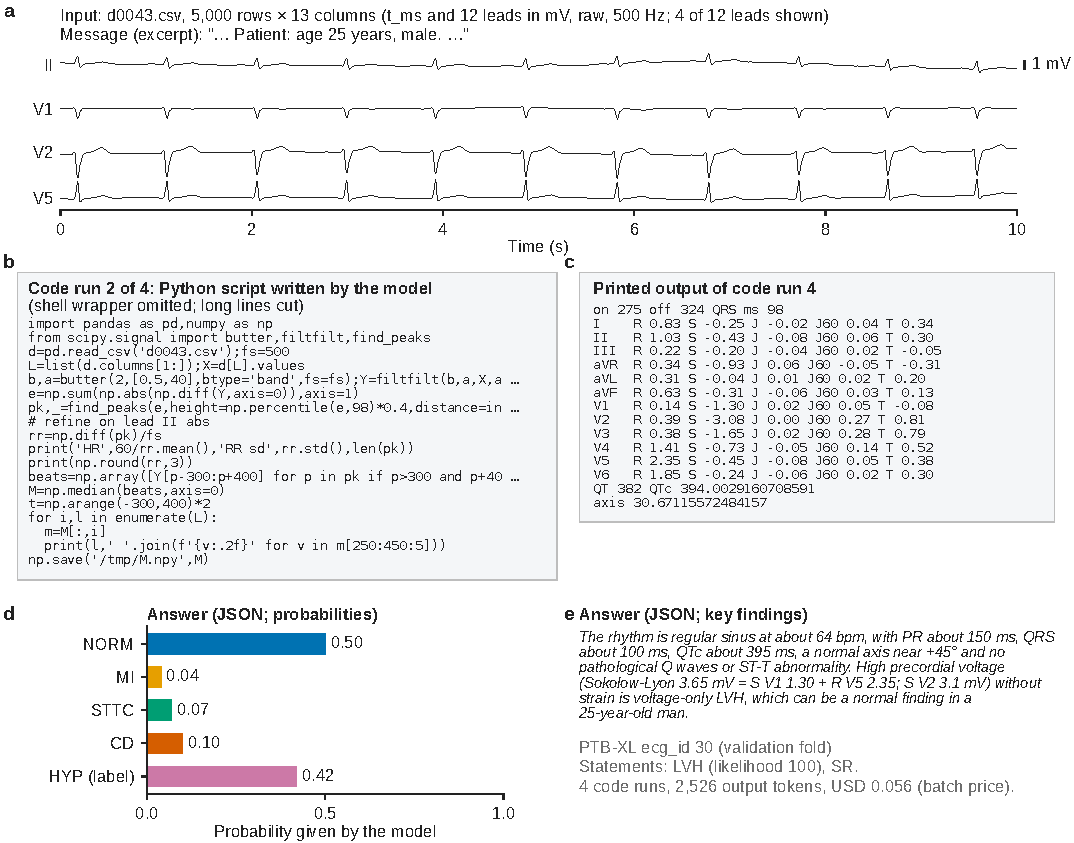
\includegraphics[width=\linewidth]{Figure_1}
  \caption{\textbf{One record from file to answer.} \textbf{a}, The input: a CSV file with the raw 10-second, 12-lead
  recording (4 of 12 leads shown; unfiltered, with baseline offsets as stored in PTB-XL), and the patient's age and sex, given
  in the user message (the complete message is in Supplementary Section~\ref{app:example}). \textbf{b}, The Python
  script of the second of \ExampleCodeRuns{} code runs, as written by the model, without its shell wrapper and with long
  lines cut (\ldots): a 0.5--40\,Hz band-pass filter, beat detection on a multi-lead envelope, RR intervals and a
  median beat per lead, whose samples it printed at 10-ms steps. \textbf{c}, The complete output of the last code run,
  as printed: QRS onset and offset (in samples) and duration (ms); per lead, R and S amplitudes, ST level at the J point
  (J) and 60\,ms later (J60) and T amplitude (mV); QT and Bazett-corrected QTc (ms) and frontal axis (degrees).
  \textbf{d}, \textbf{e}, The answer: five probabilities (``label'' marks the record's PTB-XL superclass) and the key
  findings, the answer's free-text field, which the prompt limited to two sentences. The grey note gives the record's
  PTB-XL statements (LVH, left ventricular hypertrophy; SR, sinus rhythm), code runs, output tokens and cost. The record
  (PTB-XL \texttt{ecg\_id} \ExampleECGID, validation fold) was chosen by a fixed rule, not by its result: the lowest
  \texttt{ecg\_id} whose only superclass is HYP among the validation records read with the frozen prompt. The complete
  transcript is in Supplementary Section~\ref{app:transcript}.}
  \label{fig:example}
\end{figure}

\subsection{Discrimination on the test fold}
Macro AUROC on the test fold, the primary endpoint, was \MainAUROC, with a 95\% confidence interval (CI) of
\MainAUROCLow--\MainAUROCHigh{} from \NBoot{} bootstrap resamples of the test records (see Section~\ref{sec:endpoints}), and macro average
precision (AUPRC) was \MainAUPRC. Per class, AUROC was \MainNORM{}
for NORM, \MainMI{} for MI, \MainSTTC{} for STTC, \MainCD{} for CD and \MainHYP{} for HYP (Fig.~\ref{fig:benchmark}b,
Supplementary Table~\ref{tab:perclass}; ROC and precision--recall curves in Supplementary Fig.~\ref{fig:curves}a,b).
Because the model also received the patient's age and sex, we compared it with an age-and-sex control: a logistic
regression per superclass that predicts the class from age and sex alone, fitted on the training folds (see Section~\ref{sec:endpoints}).
The control reached a macro AUROC of \AgeSexAUROC{} (Fig.~\ref{fig:benchmark}a). The model exceeded it by
$\CodeVsAgeSex$ (95\% CI $\CodeVsAgeSexLow$ to $\CodeVsAgeSexHigh$), and did so in every class (by $\CodeVsAgeSexNORM$
for NORM to $\CodeVsAgeSexHYP$ for HYP; Fig.~\ref{fig:benchmark}b). The \NTest{} test records come from
\PHNPatientsTest{} patients; \PHNPatientsMulti{} of them have two or more records, \PHNRecordsMulti{} records in
total, and records of the same patient are not independent. As a post hoc robustness check, we therefore repeated the
bootstrap on the same predictions, resampling patients with replacement, with each drawn patient contributing all of
their test records; the 95\% CI was nearly identical (\PHClusterLow--\PHClusterHigh).

Among published results on the PTB-XL superclass task (Fig.~\ref{fig:benchmark}a, Supplementary
Table~\ref{tab:benchmark}), the model's macro AUROC was \GapToBestPublishedAbs{} below the best result reported with
the same split, label definition and evaluation metric (\BestPublishedAUROC, reached by the ensemble of the original
benchmark models~\citep{Strodthoff2021} and by MultiresNet~\citep{shi2023multires}) and exceeded that of the best zero-shot
ECG--language model (\BestZeroShotAUROC~\citep{cai2025supreme}) by $\GapToBestZeroShot$. These comparisons are
informal: the published models' per-record predictions were not available, and their inputs differ (the original
benchmark models used 100\,Hz signals without age or sex).

\begin{figure}[tbp]
  \centering
  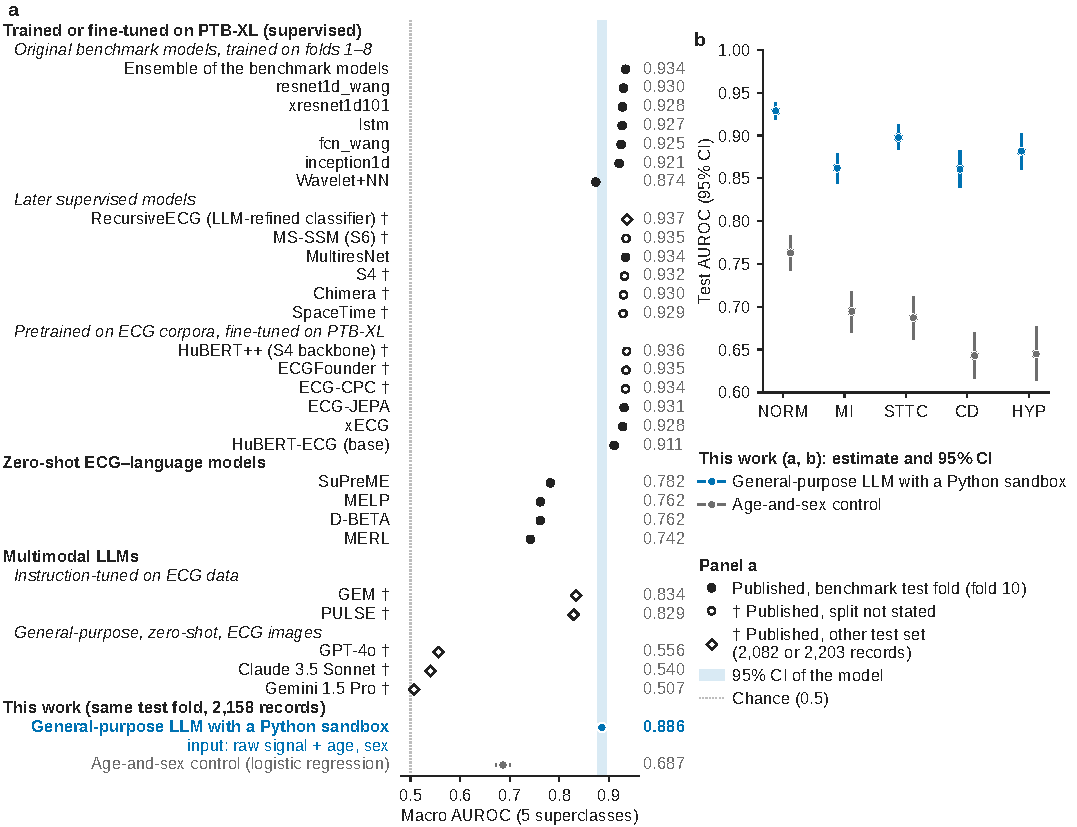
\includegraphics[width=\linewidth]{Figure_2}
  \caption{\textbf{Macro AUROC among published PTB-XL superclass results, and per class.} \textbf{a}, Published results
  as reported by their authors, grouped by model type and training (Supplementary Table~\ref{tab:benchmark} gives
  sources and inputs). Filled circles, results on the benchmark test fold (fold 10); $^\dagger$not directly
  comparable: split not stated (open circles), or a different test set (diamonds: RecursiveECG, a supervised model
  whose design an LLM agent revised, and the multimodal LLMs, including GEM~\citep{lan2025gem}). HuBERT-ECG's
  self-supervised pretraining corpus includes PTB-XL (unlabelled). This work: the LLM with a Python sandbox, which
  received the raw signal with age and sex, and the age-and-sex control, a logistic regression per class fitted on
  folds 1--8, both on all \NTest{} test-fold records with 95\% percentile bootstrap CIs (\NBoot{} resamples; the shaded
  band is the model's CI). \textbf{b}, Per-class AUROC of the model (blue) and the age-and-sex control (grey) on the
  test fold; bars are 95\% bootstrap CIs.}
  \label{fig:benchmark}
\end{figure}

\subsection{Discrimination by diagnostic statement}
We measured, post hoc, how well the model's superclass probability separated records with a given diagnostic
statement from records without that superclass (Fig.~\ref{fig:where}a, Supplementary Table~\ref{tab:statements}). This
was done for the \PHNStatements{} of PTB-XL's 44 diagnostic statements that had at least \PHMinStatement{} test
records. For example, for complete right bundle branch block, one of the statements under CD, we computed the AUROC of the model's
CD probability for the \PHStmtCRBBBN{} test records with that statement against all test records without CD. The model
gave only superclass probabilities, so this does not test whether the statement itself was identified. Separation was
best for complete right bundle branch block (AUROC \PHStmtCRBBB; \PHStmtCRBBBN{} records), complete left bundle branch
block (\PHStmtCLBBB; \PHStmtCLBBBN), left anterior fascicular block (\PHStmtLAFB; \PHStmtLAFBN), anterolateral
ischaemic change (\PHStmtISCAL; \PHStmtISCALN), anteroseptal infarction (\PHStmtASMI; \PHStmtASMIN) and non-specific
ischaemic change (\PHStmtISC; \PHStmtISCN). It was poorest for two statements defined by borderline QRS durations,
non-specific intraventricular conduction disturbance (\PHStmtIVCD; \PHStmtIVCDN) and incomplete right bundle branch
block (\PHStmtIRBBB; \PHStmtIRBBBN), and for left atrial overload (\PHStmtLAOLAE; \PHStmtLAOLAEN), inferior infarction
(\PHStmtIMI; \PHStmtIMIN) and lateral infarction (\PHStmtLMI; \PHStmtLMIN). Left ventricular hypertrophy reached
\PHStmtLVH{} (\PHStmtLVHN) and first-degree atrioventricular block \PHStmtOneAVB{} (\PHStmtOneAVBN); 95\% CIs are in
Supplementary Table~\ref{tab:statements}.

\begin{figure}[tbp]
  \centering
  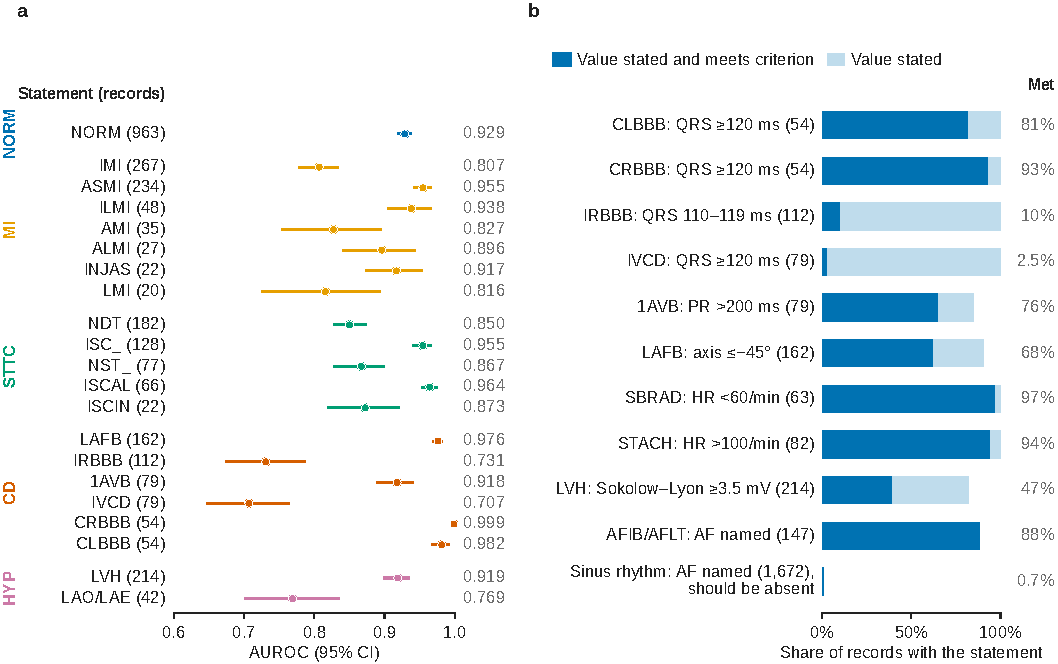
\includegraphics[width=\linewidth]{Figure_3}
  \caption{\textbf{Discrimination by diagnostic statement, and what the model stated (test fold, post hoc).}
  \textbf{a}, AUROC of the superclass probability for records with a diagnostic statement against records without that
  superclass, with 95\% stratified bootstrap CIs (\PHNStmtBoot{} resamples), for statements with at least
  \PHMinStatement{} test records, grouped by superclass (PTB-XL codes, defined below and in Supplementary
  Table~\ref{tab:statements}); number of records in brackets, AUROC at right. \textbf{b}, Measurements stated in the key
  findings of records with selected PTB-XL statements, against a criterion (number of records in brackets): light bars,
  share of all records with the statement whose key findings state the measurement; dark bars, share of all records
  with the statement whose stated value meets the criterion; at right (Met), the same share among the records that
  stated a value, as in the text and Supplementary Table~\ref{tab:measurements}. The criteria for QRS duration, PR
  interval and Sokolow--Lyon voltage are the frozen prompt's (for IVCD, QRS 120\,ms or more); the prompt gives no angle
  for fascicular block, so LAFB is shown against the AHA/ACCF/HRS criterion, an axis of $-45^\circ$ or more
  leftward~\citep{surawicz2009recommendations} ($-30^\circ$ or more in Supplementary Table~\ref{tab:measurements}).
  For the two rhythm rows (records with AFIB or AFLT, and records in sinus rhythm without them), the bar and Met give
  the share whose key findings name atrial fibrillation or flutter without negating it (AF named); in sinus rhythm, a
  short bar means agreement. Values were extracted from the text with regular expressions (Section~\ref{sec:posthoc}).
  IMI, ASMI, ILMI, AMI, ALMI, LMI: inferior, anteroseptal, inferolateral, anterior, anterolateral and lateral
  myocardial infarction; INJAS: subendocardial injury in anteroseptal leads; NDT: non-diagnostic T abnormalities;
  ISC\_, NST\_: non-specific ischaemic change and non-specific ST changes; ISCAL, ISCIN: ischaemic change in
  anterolateral and in inferior leads; CLBBB, CRBBB, IRBBB: complete left, complete right and incomplete right bundle
  branch block; IVCD: non-specific intraventricular conduction disturbance; 1AVB: first-degree atrioventricular block;
  LAFB: left anterior fascicular block; LVH: left ventricular hypertrophy; LAO/LAE: left atrial overload or
  enlargement; SBRAD, STACH: sinus bradycardia and tachycardia; HR: heart rate; AFIB, AFLT: atrial fibrillation and
  flutter.}
  \label{fig:where}
\end{figure}

\subsection{Stated measurements and the dataset's annotations}
The key findings stated a heart rate in \PHStatedCodeHr\% of test records, a QRS duration in
\PHStatedCodeQrs\%, an axis in \PHStatedCodeAxis\%, a PR interval in \PHStatedCodePr\%, a Sokolow--Lyon voltage in
\PHStatedCodeSokolow\% and a QTc in \PHStatedCodeQtc\% (post hoc; values extracted from the text with regular
expressions; see Section~\ref{sec:posthoc}). As described above, most of the stated PR intervals, QT or QTc intervals and axes appear to
have been read from printed samples rather than computed. We compared the stated values with the PTB-XL statements,
which were assigned or validated by cardiologists and are not measurements, so the comparison shows consistency, not accuracy
(Fig.~\ref{fig:where}b; the shares below are among records that stated the value, as in Supplementary
Table~\ref{tab:measurements}). Agreement was good for rate, rhythm and QRS duration in complete bundle branch block:
the stated rate was below 60/min in \PHMeasSBRADCodeCrit\% of records with sinus bradycardia and above 100/min in
\PHMeasSTACHCodeCrit\% of records with sinus tachycardia, and the stated QRS duration was 120\,ms or more in
\PHMeasCLBBBCodeCrit\% of records with complete left and \PHMeasCRBBBCodeCrit\% of records with complete right bundle
branch block. Rhythm is not part of the superclass task, but the key findings named atrial fibrillation or flutter in
\PHMeasAFCodeCrit\% of the \PHMeasAFN{} records with these rhythms and in \PHMeasSRAFCodeCrit\% of the \PHMeasSRAFN{}
records in sinus rhythm. Agreement was partial for the PR interval in first-degree atrioventricular block:
\PHMeasOneAVBCodeStated\% of these records stated one, and the stated PR exceeded 200\,ms in \PHMeasOneAVBCodeCrit\%
of those. It was also partial for the axis in left anterior fascicular block, which was $-45^\circ$ or more leftward
(the AHA/ACCF/HRS criterion~\citep{surawicz2009recommendations}) in \PHMeasLAFBFortyFiveCodeCrit\% and $-30^\circ$ or
more leftward in \PHMeasLAFBCodeCrit\%; the prompt gives no angle for fascicular block. In records labelled LVH, the
stated Sokolow--Lyon voltage met the prompt's criterion of 3.5\,mV in about half of those that stated one
(\PHMeasLVHCodeCrit\%; median \PHMeasLVHCodeMedian\,mV). Agreement was poor for incomplete right bundle branch block
(stated QRS duration 110--119\,ms in \PHMeasIRBBBCodeCrit\%) and for non-specific intraventricular conduction
disturbance (the prompt's criterion, 120\,ms or more, in \PHMeasIVCDCodeCrit\%); their median stated QRS durations
were \PHMeasIRBBBCodeMedian{} and \PHMeasIVCDCodeMedian\,ms, against \PHMeasNormQRSCodeMedian\,ms in records labelled
only NORM.

\subsection{Subgroups, calibration and the validation fold}
In post hoc subgroups (Supplementary Table~\ref{tab:subgroups}), macro AUROC was \PHSubWomen{} in
women and \PHSubMen{} in men, and \PHSubYoung{} under 50 years of age, \PHSubAgeMid{} at 50--69 years and \PHSubOld{} at
70 years or older. It was \PHSubAF{} in records with atrial fibrillation or flutter and \PHSubNotAF{} in other rhythms;
only \PHSubAFNormPos{} of the former were NORM, and the mean AUROC of the other four classes was \PHSubAFNoNorm{}
against \PHSubNotAFNoNorm. All age and rhythm strata were below the overall value (\MainAUROC); this is possible because the
overall AUROC also ranks records across strata, which differed steeply in class prevalence. Macro
AUROC was \PHSubNoise{} in records with a signal-quality flag in the PTB-XL metadata and
\PHSubNoNoise{} without, and it ranged from \PHSubDeviceMin{} to \PHSubDeviceMax{} across the \PHSubNDevices{} PTB-XL
device values with at least \PHMinSubgroup{} test records (\PHSubDeviceRecordsN{} of \NTest{} records), which are
confounded with recording sites. MI discrimination was lower when the annotator had assigned a lower likelihood to
the MI statement (post hoc; Supplementary Table~\ref{tab:subgroups}). With each MI-positive record grouped by the highest likelihood among its MI statements and
compared with all test records without MI, AUROC was \PHMILikHundred{} (\PHMILikHundredLow--\PHMILikHundredHigh) for
the \PHMILikHundredN{} records with likelihood 100, \PHMILikMid{} (\PHMILikMidLow--\PHMILikMidHigh) for the
\PHMILikMidN{} with 50--80 and \PHMILikLow{} (\PHMILikLowLow--\PHMILikLowHigh) for the \PHMILikLowN{} with 15--35;
the age-and-sex control reached \PHMILikHundredAgeSex, \PHMILikMidAgeSex{} and \PHMILikLowAgeSex{} in the same strata.
In a post hoc calibration analysis, which asks whether the probabilities can be read at face value (see Section~\ref{sec:posthoc};
Supplementary Fig.~\ref{fig:curves}c), calibration slopes of \PHSlopeMinNoCD--\PHSlopeMaxNoCD{} for NORM, MI, STTC and
HYP indicate probabilities that were not extreme enough. CD was close to calibrated, with a slope of \PHSlopeCD{} and an expected calibration error (ECE) of \PHECECD. MI was
underestimated in every probability bin above the lowest (overall mean probability \PHMeanPMI{} against a prevalence
of \PHPrevMI), and HYP was overestimated (\PHMeanPHYP{} against \PHPrevHYP). The mean ECE over the five classes was
\PHECEMean{} and the mean Brier score \PHBrierMean.

On the validation fold, the frozen prompt had reached \DevVTwo{} (\DevVTwoLow--\DevVTwoHigh) on the 500 records on
which it was chosen and \DevFreshVTwo{} (\DevFreshVTwoLow--\DevFreshVTwoHigh) on the 200 records used only to compare
it with the last variant, so selection on the 500 records does not explain the lower test result (\MainAUROC). The
validation records were easier for the age-and-sex control (\DevAgeSexAll{} on these \NDevVTwoAll{} records and
\DevAgeSexFold{} on the whole validation fold, both post hoc, against \AgeSexAUROC{} on the test fold). No record was run
twice, so run-to-run variability, which could contribute to the difference between the validation and test results,
was not assessed.

\section{Discussion}

On the first question, a general-purpose LLM that received raw 12-lead recordings as files and processed them with code it wrote itself
classified PTB-XL ECGs into the five diagnostic superclasses with a macro AUROC of \MainAUROC{} on the benchmark test
fold, without ECG-specific training, retrieval, labelled examples or class prevalences in the prompt, and every record
received an answer. It exceeded the control that used only age and sex by $\CodeVsAgeSex$ and is
\GapToBestPublishedAbs{} below the best published result with the same split, label
definition and metric, reached by a supervised ensemble~\citep{Strodthoff2021} and by MultiresNet~\citep{shi2023multires},
both trained on the labelled training folds. In an
informal comparison, the result exceeds the best zero-shot ECG--language model~\citep{cai2025supreme} by
$\GapToBestZeroShot$; that model was pretrained on hundreds of thousands of ECGs with report-derived labels. In other
studies, general-purpose LLMs that were given ECG images or numeric series as text, including recent models, have scored near
chance or missed most critical findings~\citep{liu2024teach,seki2025assessing,ahammad2026ecgimage,soubh2026performance,gao2026luminaecg,liu2025picture,langer2025opentslm}.

On the second question, the transcripts, analysed post hoc, show how the model used the sandbox. It wrote code to filter the signal and detect
beats in every record and to form median beats in almost every record, but it rarely printed the full measurement
table that the prompt asked for. Its code usually printed a heart rate, but for most of the PR intervals, QT or QTc
intervals and axes that the model stated, no value was printed under the measurement's own label, and a Sokolow--Lyon sum
was almost never printed. The printed median-beat samples suggest that the model read these
intervals and axes from samples of the median beats it had built. The sandbox thus appears to have served less to
replace reading with computation than to give the model median beats of its own making from the full recording, in the
leads, segments and resolution it chose. Our data cannot show why the model departed from the prompt, but two
observations bear on it. The values printed most often under their own label were those that follow directly from beat
detection (heart rate in \PHPrintedHrPct\% of records, QRS duration in \PHPrintedQrsPct\%). The PR and QT intervals,
printed in \PHPrintedPrPct\% and \PHPrintedQtcPct\%, require locating the onset of the P wave and the end of the T wave,
which is harder to do automatically~\citep{martinez2004wavelet}; in a challenge on QT measurement, the best automated
method erred more than twice as much as the best manual one~\citep{moody2006qt}. The axis and the Sokolow--Lyon voltage
are simple sums of amplitudes that the model could form from a printed per-lead amplitude table (\PHLeadAmplitudePct\%
of records). Moreover, the prompt asked for a table of more than 20 measurements, eight of them for every lead, and
LLMs satisfy fewer of an instruction's requirements as their number grows~\citep{jiang2024followbench}. Because the
model sees only what its code prints, a value computed but not printed could not inform the answer; each stated value
came from printed output or from the model's own reading of printed numbers.

On the third question, the superclass probabilities, analysed post hoc by diagnostic statement, best separated records
with complete
bundle branch blocks, left anterior fascicular block, anterolateral or non-specific ischaemic change or anteroseptal
infarction from records without the superclass (AUROC \PHStmtASMI--\PHStmtCRBBB). They did so least well for
incomplete right bundle branch block and non-specific intraventricular conduction disturbance (\PHStmtIRBBB{} and
\PHStmtIVCD), two statements defined by borderline QRS durations. This measures how well the superclass probability
separated these records, not whether the statement itself was identified. For these two statements, the QRS durations
that the model stated rarely met the prompt's criteria (110--119\,ms in \PHMeasIRBBBCodeCrit\% and 120\,ms or more in
\PHMeasIVCDCodeCrit\% of the records).

The remaining gap to supervised networks is unlikely to reflect missing information in the recordings, since networks
trained on the same recordings reach \BestPublishedAUROC~\citep{Strodthoff2021}. A zero-shot model can apply only the
criteria it is given or knows, and PTB-XL's labels reflect the annotators' practice as well as textbook thresholds. In
post hoc analyses (Supplementary Table~\ref{tab:subgroups}), MI discrimination fell from \PHMILikHundred{} to \PHMILikLow{} as the highest likelihood that the
annotator assigned to a record's MI statements fell from 100 to 15--35. Part of this fall is expected for any
classifier (the age-and-sex control also fell, from \PHMILikHundredAgeSex{} to \PHMILikLowAgeSex), and without
per-record predictions of supervised networks we did not test whether theirs falls less. Among records labelled left
ventricular hypertrophy (LVH) whose key findings stated a Sokolow--Lyon voltage, about half (\PHMeasLVHCodeCrit\%)
stated 3.5\,mV or more (median \PHMeasLVHCodeMedian\,mV); LVH labels may rest on other criteria or on the annotators'
judgement. Supervised models may learn such labelling conventions from the labels, but this is a hypothesis that our data
cannot test. The stated measurements may also reflect the 0.5--40\,Hz filter that the model chose in every record: an
upper cutoff of 40\,Hz, far below the 150\,Hz recommended for diagnostic ECGs in
adults~\citep{kligfield2007recommendations}, can reduce QRS amplitudes and blur QRS onset and offset. In the
development runs, labelled examples attached as files did not measurably improve on the frozen prompt: on the same
100 records, macro AUROC was \DevBoth{} with them and \DevVTwoHundred{} without, a paired difference of
$\DevBothDiff$ ($\DevBothDiffLow$ to $\DevBothDiffHigh$) that was computed after the freeze from the same runs. Nor did
rules for PTB-XL's labelling conventions (Table~\ref{tab:development}), although the samples were small.

Each answer came with the code the model ran, what the code printed and the key findings, and the complete transcript of
every request is part of the released data. These records make the model's work inspectable in a way that class
scores are not: a reader can check how the signal was filtered, how the beats were detected and what was printed, as in
Fig.~\ref{fig:example}. They can also be checked by execution: replayed offline, the model's code reproduced the
printed output of the API's sandbox in all \RPRuns{} code runs, up to floating-point rounding, the order of tied
values and a randomly named directory. This confirms the computations behind each answer, not that the model would write the same code again. The
records document how the median beats were formed more fully than how each stated value was
obtained, because most stated PR intervals, QT or QTc intervals and axes appear to have been read from printed samples
rather than computed, and the stated values were rounded and sometimes differed from printed ones. On the second part of the third question, the stated values, compared post hoc,
were consistent with the cardiologists' statements for rate, rhythm and QRS duration in
complete bundle branch block, partly for the PR interval in first-degree atrioventricular block and the axis in left
anterior fascicular block, for about half of the LVH records that stated a Sokolow--Lyon voltage, and poorly for
incomplete right bundle branch block and non-specific intraventricular conduction disturbance. The consistency for rate,
rhythm and complete bundle branch block suggests that the key findings were specific to each recording. However,
consistency with categorical statements is not accuracy: the stated values were not compared with reference
measurements, such as those that ECG software provides for PTB-XL~\citep{Strodthoff2023ptbxlplus}. The reasoning
returned by the API is a summary, and we did not test whether the stated measurements determined the probabilities.

For practice, the approach needs no labelled data for model training, although the prompt was developed on
\NDevRecordsUsed{} labelled validation records; it needs only a general-purpose LLM with a Python sandbox and a prompt.
In the configuration tested here, the approach is currently not ready for clinical use. Discrimination was below that of trained networks, the superclass task is coarse and
leaves out rhythm diagnoses, the probabilities would need recalibration, and the model did not follow its measurement
instructions reliably. Inference currently costs about USD \CostPerRecord{} per ECG at batch prices (USD \CostPerThousand{}
per thousand; Supplementary Section~\ref{app:cost}), far more than running a trained network, and the batch interface returns results after a delay. Sending raw
ECGs to an external service requires data-governance arrangements, and clinical use would require prospective
validation and review of errors by cardiologists. A potential advantage, not tested here, is that the same model can be
redirected to other criteria or tasks by changing the prompt rather than by retraining.

Beyond these limitations of the approach, the study itself has limitations. It used one public dataset. PTB-XL and its labels have been public since
2020~\citep{Wagner2020} and derived measurements since 2023~\citep{Strodthoff2023ptbxlplus}, all before the model's
training-data cutoff (June 2026~\citep{anthropic2026models}). The model knew that it was classifying PTB-XL records,
because the prompt names PTB-XL's superclasses, and it had some knowledge of the dataset: the API returned a non-empty
reasoning summary for \PHSummariesNonEmptyN{} of \NTest{} records, and \PHThinkPTBXLN{} of these
(\PHThinkPTBXLNonEmptyPct\%) mentioned PTB-XL by name (post hoc), mostly its labelling conventions. In the example shown in Fig.~\ref{fig:example}, the model reasoned
that voltage-only LVH is often labelled as LVH in datasets like PTB-XL (reasoning summary in Supplementary
Section~\ref{app:transcript}). The
files carried anonymous names and no identifiers, so the model could not look a record up by name, but we cannot exclude
that exposure to PTB-XL or to work that used it during training affected the result. The setting is zero-shot in a
narrow sense: the model's parameters were not updated and the prompt contained no labelled examples or class
prevalences, but the prompt defines the superclasses as PTB-XL does, and the configuration was chosen on labelled
validation records. In this configuration, the test fold was read once, by one model from one vendor. No configuration of this model without the sandbox is reported
here, so the study does not show how much of the result is due to the sandbox itself. Outputs are not deterministic, no repeat runs were made, and the confidence
intervals reflect the sampling of records only. Variants of the frozen prompt were compared on 100 or 200 records, where
the 95\% CIs of the paired differences had half-widths of about \DevFreshVFiveDiffHalfWidth{} (200 records) and
\DevBothDiffHalfWidth--\DevStatementsDiffHalfWidth{} (100 records), so differences of about that size or smaller could
not be reliably detected. The diagnostic criteria in the prompt are condensed and in places simplified (Supplementary
Table~\ref{tab:criteria}): poor R-wave progression is listed for MI although it is not a diagnostic criterion, long
QTc is listed under STTC, as PTB-XL classifies it, although it is not specific to ischaemia, the threshold for
non-specific intraventricular conduction disturbance is higher than the recommended one, and the age- and
sex-specific thresholds for ST elevation in V2--V3 and most criteria for RVH are not given. Whether criteria stated as
in the guidelines would improve discrimination was not tested; it would need new development runs. It should be
noted that the comparisons with published results (Fig.~\ref{fig:benchmark}a)
are informal, because inputs (sampling rates; age and sex,
which only this model received) and in some cases splits differ and per-record predictions were not available. The
measurements were extracted from free text with regular expressions, and the statements they were compared with are
categorical labels of a single annotation process that, following the benchmark definition, include statements of any
likelihood. The analysis of what the model did in the sandbox, the per-statement results, the subgroups, the calibration
analysis, the MI likelihood strata, the patient-level bootstrap, the age-and-sex control on the validation fold, the
measurement analysis, the count of PTB-XL mentions in the reasoning summaries and the local replay of the model's code
were added after the test run.

Evaluation on ECGs recorded after the model's training-data cutoff would address both generalization and possible exposure
to PTB-XL. Comparing the stated measurements with reference measurements, diagnostic criteria stated as in the guidelines,
prompts or tools that make the model compute
its measurements in code, having cardiologists review the transcripts of errors, stratifying the predictions of a
supervised network by annotation likelihood, extending the approach to PTB-XL's finer diagnostic and rhythm
tasks~\citep{Strodthoff2021}, repeating runs and testing LLMs from other vendors would show how far the approach
extends and how far its written work can be trusted.

In conclusion, given a Python sandbox and raw 12-lead recordings, a general-purpose LLM processed each ECG with its own
code and classified the PTB-XL superclasses with a macro AUROC of \MainAUROC{} without training on labelled ECGs,
between published zero-shot ECG--language models and supervised networks. It used code mainly to prepare median
beats, and its transcripts suggest that it read most of the intervals and axes it stated from samples it printed;
every answer came with the code the model ran, what the code printed and the measurements the model stated.

\section{Methods}\label{sec:methods}

\subsection{Study design}
This is a retrospective evaluation of a general-purpose LLM with a Python sandbox, used as a zero-shot classifier of
12-lead ECGs on a public dataset; the model was blind to labels and PTB-XL identifiers. We use zero-shot to mean that
the model's parameters were not updated (no training or fine-tuning), that the prompt contained no labelled examples
and no class prevalences, and that no retrieval of external information was used. The prompt did define the superclasses as PTB-XL does, and
the configuration was developed on labelled validation records (``Development and freeze''). The input format,
prompt, model settings and analysis plan were fixed in a written protocol that was frozen before the test fold was
run. Analyses added after the test run are listed under ``Post hoc analyses'' below and labelled post hoc where they
are reported. Ethics is described at the end of this section.

\subsection{Data, labels and split}
We used PTB-XL version 1.0.3~\citep{Wagner2020,Wagner2022physionet} (\NRecordsTotal{} records from \NPatients{}
patients, 10\,s, 12 leads, recorded between October 1989 and June 1996 at 400\,Hz and resampled to 500\,Hz by the
dataset's authors; the dates in the metadata are shifted per patient). PTB-XL annotates each record with statements
of the SCP-ECG standard (Standard Communication Protocol for Computer-Assisted Electrocardiography) and gives each
diagnostic statement a likelihood from 0 to 100, inferred from keywords in the ECG report that express the
cardiologist's certainty (0 where the report gave no such information)~\citep{Wagner2020}. Labels and split follow the
public benchmark~\citep{Strodthoff2021}: every diagnostic SCP-ECG statement of a record (as marked in PTB-XL's
\texttt{scp\_statements} table) contributes its diagnostic superclass (NORM, MI, STTC, CD or HYP), irrespective of its
likelihood; records without any superclass are removed, which leaves \NWithSuperclass{} records. All test-fold records
are marked in PTB-XL as validated by a human annotator. A record can have several superclasses. Folds 1--8
(\NTrain{} records) form the benchmark training set, fold 9 (\NVal{} records) the validation set and fold 10
(\NTest{} records) the test set; no patient appears in more than one of these sets (Supplementary
Table~\ref{tab:characteristics}). All development runs used fold 9. Folds 1--8 were used only to fit the age-and-sex
control, to compute the class prevalences reserved for failed records, and for the labelled example files tried
during development. In this study, the test fold was used only for the frozen test run, the pre-specified evaluation
and, after the test run, the post hoc analyses.

\subsection{Input}
Each record was written to a CSV file with a time column in milliseconds and the 12 leads (I, II, III, aVR, aVL, aVF,
V1--V6) in millivolts with three decimals, one row per sample: the full 10-second recording at 500\,Hz (5{,}000 rows),
unfiltered, as stored in PTB-XL. We call this input raw: the digital signal as distributed in PTB-XL (after the
recording devices' own processing and the dataset authors' resampling), with no filtering, baseline correction, beat
detection or feature extraction by us. Three decimals in millivolts keep PTB-XL's resolution of 1\,\textmu V. The file was uploaded through the API's Files interface and attached to the request,
which made it available in the sandbox. The user message named the file and gave the patient's age and sex (ages of 90
years or more, which PTB-XL codes as 300, as ``90 or older''); Supplementary Section~\ref{app:example} shows one
message. No derived measurement, filter, report or label was provided.

\subsection{Model, sandbox, prompt and inference}\label{sec:inference}
We used \ModelID{} through the Anthropic Messages API with the server-side code-execution tool
(\CodeTool): a sandboxed container in which the model can run shell commands and Python (with NumPy, SciPy and pandas)
on the attached file, without internet access~\citep{anthropic2026codeexec}. Within one request, each code run is one round: the model
writes code, the sandbox executes it and returns the printed output, and the model then either runs more code or
answers. The prompt asked for measurement before judgement but did not set the number of runs. The API pauses a
request after a set number of tool rounds, and the protocol allowed up to two continuations in the same container. In the test run, each
request ran in a container of its own. Reasoning effort was \Effort{}, the output limit was \MaxTokens{} tokens per
API call (including reasoning, code and answer), and adaptive thinking was used with summarized display, so the API
returned a summary of the model's reasoning; in the test run this summary was empty for many requests, although every
request had used reasoning tokens (see (viii) under ``Post hoc analyses''). The model exposes no sampling parameters
(no temperature or seed), so outputs are not deterministic. The provider controls the sandbox image; error tracebacks
show Python 3.11, and package versions were not recorded. The model's published training-data cutoff is June
2026~\citep{anthropic2026models}. Development runs were the trial runs on validation-fold records in which prompts were
compared and the frozen prompt was chosen (``Development and freeze''); the test run was the single run of the frozen
prompt on the test fold. Development runs were made from \DevFirstSubmitUTC{} UTC on
\DevFirstSubmitDateLong{} to \DevLastCollectUTC{} UTC on \DevLastCollectDateLong, and the test run between
\TestFirstSubmitUTC{} and \TestLastCollectUTC{} UTC on \TestRunDateLong.

The system prompt (Supplementary Section~\ref{app:prompt}, SHA-256 prefix \PromptSHA) assigns the role of a
cardiologist with a Python sandbox, describes the file, and asks the model to work in two steps. In the first, it
filters the signal, detects beats, forms a median beat per lead with the baseline set from the PR segment, and
computes and prints a complete measurement table (rhythm, rate and regularity; PR, QRS duration from the earliest
onset to the latest offset over all leads, QT, and QTc by Bazett's formula; frontal axis; per lead, Q-wave duration
and depth, R, S and R$'$ amplitudes, ST level at the J point and 60\,ms later and T amplitude; the
Sokolow--Lyon~\citep{Sokolow1949} and Cornell~\citep{Casale1985,Casale1987} voltages and R in aVL; P-wave amplitude,
duration and terminal negativity in V1), and re-measures implausible values. In the second, it applies criteria for
each superclass to the table, weighing the overall pattern. The criteria were written for this study as a condensed
list of commonly used thresholds, not taken from a single source; Supplementary Table~\ref{tab:criteria} gives the
closest published criterion for each, from the AHA/ACCF/HRS recommendations for the interpretation of the
ECG~\citep{surawicz2009recommendations,rautaharju2009recommendations,hancock2009recommendations,wagner2009recommendations},
the fourth universal definition of myocardial infarction~\citep{thygesen2018fourth}, the guideline on bradycardia and
conduction delay~\citep{kusumoto2019bradycardia} and the original voltage criteria~\citep{Sokolow1949,Casale1985},
and marks where the prompt departs from it. The prompt defines the five superclasses as
in PTB-XL, states that rhythm findings alone are not superclass labels, and says that discrimination is measured, so
that probabilities should reflect graded evidence. It contains no class prevalences and no examples. The output was
constrained by a JSON schema (Supplementary Section~\ref{app:schema}): the record identifier, the key findings (free
text, which the prompt limits to at most two sentences naming the decisive findings and measurements) and five
independent probabilities.

Each record was sent as its own request through the Message Batches interface. The system prompt was identical across
requests and marked for prompt caching. The API reported the token counts of every request, from which cost was
computed at the provider's list prices (Supplementary Section~\ref{app:cost}).

\paragraph{Blinding.} Records were shuffled (seed 7) and given anonymous identifiers, which were also the file names;
the mapping to PTB-XL identifiers was stored locally and was never part of any request in the development or test
runs. The model saw no labels, reports or PTB-XL identifiers of the records it classified.

\subsection{Development and freeze}
The configuration was developed on the validation fold (fold 9) in \NDevRuns{} development runs. Each prompt was run
once on each set of records, and prompts were compared by macro AUROC against the validation labels:
\begin{enumerate}
  \setlength{\itemsep}{0pt}\setlength{\parsep}{0pt}
  \item A first, basic prompt asked the model to analyse the ECG as a cardiologist would and to measure whatever it
  judged necessary, without a measurement list or diagnostic criteria. It was run on 500 fold-9 records drawn at
  random (\texttt{protocol/dev500\_ids.txt}).
  \item The frozen prompt replaced this with the two steps described above: a fixed list of measurements to compute
  and print, then written criteria for each superclass. On the same 500 records it reached \DevVTwo{} (95\% CI
  \DevVTwoLow--\DevVTwoHigh). This was the only change that gave a measurable gain.
  \item Three variants of the frozen prompt were each compared with it on the same records by a paired bootstrap
  (Table~\ref{tab:development}): (a) ten labelled example recordings attached as files with their labels, two per
  superclass, taken from the training folds (1--8) so that no validation or test record served as an example (on 100
  of the 500 records, drawn at random); (b) probabilities for PTB-XL's 44 diagnostic statements instead of the five
  superclasses, aggregated to superclasses by their maximum (the same 100 records); and (c), after an error analysis
  on the 500 records, added rules for PTB-XL's labelling conventions (on 200 fold-9 records not used before, on which
  the frozen prompt reached \DevFreshVTwo, 95\% CI \DevFreshVTwoLow--\DevFreshVTwoHigh). None of them improved on the
  frozen prompt.
\end{enumerate}
The frozen prompt was kept because of the gain in step 2, because no variant improved on it, and because it needs no
labelled examples; it contains no training-fold data. All prompts are in \texttt{prompts/}. Development used
\NDevRecordsUsed{} distinct fold-9 records (the 500-record sample, the 200 new records and \NPilotExtra{} further
records from a \NPilot-record pilot whose other \NPilotInMain{} were in the 500-record sample) and cost
USD \DevCostTotal.

\begin{table}[tbp]
  \centering
  \caption{\textbf{Development on the validation fold (fold 9).} Each variant of the frozen prompt was run on the same
  records as the frozen prompt; macro AUROC and paired differences (variant minus frozen prompt) with 95\% percentile
  bootstrap CIs (\NBoot{} resamples). The 100 records are a random subset of the 500-record sample; on all 500, the
  frozen prompt reached \DevVTwo{} (95\% CI \DevVTwoLow--\DevVTwoHigh). The 200 records had not been used in
  development before. Each prompt was run once on each set of records; the CIs come from resampling the records
  (bootstrap), not from repeated runs. All runs were made before the freeze. The difference in the first row (the frozen prompt with the example files)
  was computed after the test run (post hoc).}
  \label{tab:development}
  \small
  \begin{tabular}{lrccc}
    \toprule
     & & \multicolumn{2}{c}{Macro AUROC} & \\
    \cmidrule(lr){3-4}
    Change & Records & Frozen prompt & Variant & Difference [95\% CI] \\
    \midrule
    + 10 labelled example files & 100 & \DevVTwoHundred & \DevBoth &
      $\DevBothDiff$ [$\DevBothDiffLow$, $\DevBothDiffHigh$] \\
    Statement-level output & 100 & \DevVTwoHundred & \DevStatements &
      $\DevStatementsDiff$ [$\DevStatementsDiffLow$, $\DevStatementsDiffHigh$] \\
    + rules for labelling conventions & 200 new & \DevFreshVTwo & \DevFreshVFive &
      $\DevFreshVFiveDiff$ [$\DevFreshVFiveDiffLow$, $\DevFreshVFiveDiffHigh$] \\
    \bottomrule
  \end{tabular}
\end{table}

The code, configuration and prompts were then frozen together with a written protocol that records
the prompt's SHA-256 hash, the endpoints and the analysis plan. The software refuses to build a test-fold run unless
the code, configuration and prompts are unchanged since the freeze and no experimental setting other than the
record-shuffle seed differs from the frozen configuration; the test-run manifest records no difference from the frozen
configuration, including the seed (7). The protocol was not registered externally.

\subsection{Test run and failure handling}
The \NTest{} test requests were sent in \NBatches{} batches of at most 250, one after another, with pre-specified stop
rules (a batch costing more than USD 20 or with more than 10\% failed answers). An answer had to contain five finite
probabilities; failed requests were to be retried once, requests paused by the API resumed up to twice, and records
still without an answer were to be given the training-fold class prevalences, with their number reported. None of
these was needed: no stop rule was triggered, and every request in the \NBatches{} batches returned a valid answer at
the first attempt. Every paid request was logged with its token counts and cost.

\subsection{Endpoints and statistical analysis}\label{sec:endpoints}
The pre-specified primary endpoint was macro AUROC over the five superclasses (scikit-learn \texttt{roc\_auc\_score},
macro average), the benchmark's metric~\citep{Strodthoff2021}, on all \NTest{} test records from the single test
run, with a 95\% percentile bootstrap confidence interval (CI)~\citep{Efron1993} (\NBoot{} resamples of records, seed 0,
keeping only resamples with positives and negatives of every class). Pre-specified secondary endpoints were per-class
AUROC, macro average precision (AUPRC), code runs, tokens and cost per record, and paired differences in macro AUROC,
computed on the same bootstrap resamples, against a logistic regression per class on age, age squared and sex (ages
coded 300 entered as 90), fitted on folds 1--8. Results of published models were compared as reported
by their authors, without significance tests. Per-class confidence intervals and per-class differences from the control use the same resamples and were not
pre-specified.

\subsection{Post hoc analyses}\label{sec:posthoc}
After the test run we added the following analyses.
\begin{enumerate}
  \renewcommand{\labelenumi}{(\roman{enumi})}
  \setlength{\itemsep}{0pt}\setlength{\parsep}{0pt}
  \item What the model did in the sandbox, from the transcripts: the non-empty lines of code per record; the code runs
  that ended with an error (a non-zero exit status, or an uncaught Python exception other than a broken pipe in the
  error output, since piped commands return the exit status of the last command) and, in records with an error,
  whether the last code run succeeded; whether the code called a filter (and its cutoffs), a peak detector and a
  median function; and whether the printed output contained the labels of heart rate, QRS, PR, QT or QTc, axis and
  Sokolow--Lyon voltage, a per-lead table of R and S amplitudes, or lines of 20 or more numbers. A printed label shows
  that a labelled value was printed, not where a stated value came from.
  \item Discrimination by diagnostic statement, for statements with at least \PHMinStatement{} test records, as the
  AUROC of the superclass probability for records with the statement against records without the superclass, with
  95\% CIs from \PHNStmtBoot{} stratified bootstrap resamples; this measures how well the superclass probability
  separated these records, not whether the statement itself was identified.
  \item Subgroups by sex, age (under 50 years, 50--69 years, 70 years or older), rhythm (atrial fibrillation or
  flutter), signal-quality flags and extra beats noted in the PTB-XL metadata, and recording device (the device values
  as recorded in PTB-XL, with at least \PHMinSubgroup{} test records); for the rhythm subgroups also as the mean AUROC
  of the four classes other than NORM, which had few positive records in atrial fibrillation or flutter.
  \item Calibration, that is, whether the probabilities can be read at face value (of records given a probability of
  about 0.3 for a class, about 30\% should have it). AUROC depends only on how records are ranked, so it does not
  measure this. We report the expected calibration error (ECE: the absolute gap between mean predicted probability and
  observed frequency in ten equal-width probability bins, averaged with weights by the number of records per bin), the
  Brier score (the mean squared difference between probability and label) and the calibration slope (the slope of a
  logistic regression of the label on the log-odds of the probability: 1 for calibrated probabilities, above 1 for
  probabilities that are not extreme enough).
  \item MI discrimination by the likelihood of the MI statements: each MI-positive record was grouped by the highest
  likelihood among its MI statements (100; 50--80; 15--35) and compared with all test records without MI, with 95\% CIs
  from \PHNStmtBoot{} stratified bootstrap resamples as in (ii); the age-and-sex control was evaluated on the same
  groups.
  \item A bootstrap that resampled patients with replacement instead of records, each drawn patient contributing all
  of their test records (\NBoot{} resamples), because records of the same patient are not independent.
  \item The measurements stated in the key findings, that is, the values that the model wrote in the answer's free
  text, whatever their source: heart rate, PR, QRS duration, QTc, axis and Sokolow--Lyon voltage. The key findings of
  the record in Fig.~\ref{fig:example}e, for example, state all six, among them an axis near $+\ExampleAxisStated^\circ$,
  whereas the code had printed an axis of $\ExampleAxisPrinted^\circ$ (Fig.~\ref{fig:example}c). They were extracted
  from the key-findings text with regular expressions (the first value with its unit after the
  measurement's label within its clause; the midpoint of a stated range; for Sokolow--Lyon the stated sum, not a
  component; details in Supplementary Table~\ref{tab:measurements}), and mentions of atrial fibrillation or flutter
  were detected with a pattern that excluded negations. These were tabulated against the PTB-XL statements and the
  heart-axis field of the PTB-XL metadata, with the criteria of the frozen prompt where it gives one (QRS 120\,ms or
  more for complete bundle branch block and non-specific intraventricular conduction disturbance, 110--119\,ms for
  incomplete right bundle branch block, PR over 200\,ms for first-degree atrioventricular block, Sokolow--Lyon voltage
  3.5\,mV or more for left ventricular hypertrophy) and conventional limits otherwise. The prompt gives no angle for
  fascicular block, so the stated axis in left anterior fascicular block was compared with two thresholds, $-30^\circ$
  (left axis deviation) and $-45^\circ$ (the AHA/ACCF/HRS criterion~\citep{surawicz2009recommendations}).
  \item Mentions of PTB-XL by name in the reasoning summaries, among the \PHSummariesNonEmptyN{} of \NTest{} test
  records whose summary was not empty.
  \item Two analyses on the validation fold: the age-and-sex control on the \NDevVTwoAll{} records read with the frozen
  prompt and on the whole fold, and the paired difference of the example-file variant from the frozen prompt (first
  row of Table~\ref{tab:development}), computed from development runs made before the freeze.
  \item A local replay of the model's code: every code run of the test run was executed again, record by record and
  in the original order, on a local computer without network access, in a sandbox (bubblewrap) that mirrored the API
  container: the record's file was in the directory named by the same environment variable, and working files were
  kept across the runs of one record. It used Python \RPPython{} with NumPy \RPNumPy, SciPy \RPSciPy, pandas
  \RPPandas{} and matplotlib \RPMatplotlib, chosen to match what the tracebacks and printed output show (Python 3.11,
  NumPy 2). The printed output of each run was compared with the output the API returned and classed as identical,
  equal up to rounding (the same text, with every number within one unit of its last printed digit or within a
  relative $10^{-9}$) or different; an error as defined in (i) counted as reproduced if the local run also ended with
  an error of the same exception type. The model was not queried again, so the replay tests the code runs, not the
  model's answers.
\end{enumerate}

\subsection{Software}
Local analyses used Python 3.13.9 with NumPy 2.3.5, SciPy 1.16.3, pandas 2.2.3, scikit-learn 1.7.2, wfdb 4.3.1,
matplotlib 3.10.6 and the Anthropic Python SDK 0.117.0; the exact versions of the packages that the code uses directly
are pinned in \texttt{requirements-lock.txt}.

\subsection{Ethics}
This is a secondary analysis of PTB-XL~\citep{Wagner2020,Wagner2022physionet}, a public, de-identified dataset; no new
data were collected and no participant was contacted. The PTB-XL authors report that their institutional ethics
committee approved the publication of the anonymous data in an open-access database (PTB-2020-1), and that personal
information in the metadata was pseudonymized and recording dates were shifted by a random offset per
patient~\citep{Wagner2020,Wagner2022physionet}. This analysis therefore required no further ethics approval, and none
was sought. The de-identified recordings were processed through a commercial API (Anthropic).

% Input directly after sections/04_methods: the \subsection entries below continue the Methods section
% (npj Digital Medicine asks for ethics details in the Methods). The unnumbered sections
% after them are the end matter, in the journal's order, before the references.

\subsection{Ethics}
This is a secondary analysis of PTB-XL~\citep{Wagner2020,Wagner2022physionet}, a public, de-identified dataset; no new
data were collected and no participant was contacted. The PTB-XL authors report that their institutional ethics
committee approved the publication of the anonymous data in an open-access database (PTB-2020-1), and that personal
information in the metadata was pseudonymized and recording dates were shifted by a random offset per
patient~\citep{Wagner2020,Wagner2022physionet}. This analysis therefore required no further ethics approval, and none
was sought. The de-identified recordings were processed through a commercial API (Anthropic).

\section*{Data availability}
PTB-XL 1.0.3~\citep{Wagner2022physionet} is available from PhysioNet~\citep{Goldberger2000,Pollard2026}
(\url{https://doi.org/10.13026/kfzx-aw45}) under the Creative Commons Attribution 4.0 International License. The
derived data of this study, the complete run folders of the test run and of all development runs, are attached as an
archive to release v1.0 of the project repository (Code availability): for every request, the request and the result, with the complete sandbox transcript (the code the model ran
and its printed output), the summarized reasoning, the answer, token counts and cost; per-record predictions; the
mapping from anonymous identifiers to PTB-XL identifiers; and usage summaries, batch logs and run manifests.

\section*{Code availability}
Code, prompts and the scripts that produce all tables, figures and results in this paper are
publicly available at \url{https://github.com/piculjantechnologies/ecg-llm-code} under the MIT licence;
release v1.0 is the version described here. The analysis
scripts in \texttt{analysis/} were written after the test run; the pre-specified endpoints are computed with the frozen
evaluation code. All API calls are isolated in one module (\texttt{ecgcode/api.py}); every other step, including
evaluation, runs offline.

% End matter before the references, in the journal's order (Data and Code availability are in 05_statements).

\section*{CRediT authorship contribution statement}
\textbf{Neven Pi\v{c}uljan:} Conceptualization, Methodology, Software, Investigation, Formal analysis, Data curation,
Visualization, Resources, Writing -- original draft, Writing -- review \& editing. \textbf{Alan Jovi\'c:} Methodology,
Validation, Supervision, Writing -- review \& editing. Both authors read and approved the final manuscript.

\section*{Declaration of competing interest}
The authors have no employment, grant, API-credit, shareholding or other relationship with Anthropic, whose model is
evaluated in this study, and declare no other financial or non-financial competing interests.

\section*{Funding}
This research did not receive any specific grant from funding agencies in the public, commercial, or not-for-profit
sectors. Pi\v{c}uljan Technologies paid all API costs.

\section*{Declaration of generative AI and AI-assisted technologies in the manuscript preparation process}
During the preparation of this work Neven Pi\v{c}uljan used Claude Opus 5.5 to assist with writing and editing the
manuscript and the analysis code. After using this tool, the authors reviewed and edited the content as needed and take full
responsibility for the content of the published article.


\bibliographystyle{unsrtnat}
\bibliography{refs}

\end{document}
